% Options for packages loaded elsewhere
\PassOptionsToPackage{unicode}{hyperref}
\PassOptionsToPackage{hyphens}{url}
\PassOptionsToPackage{dvipsnames,svgnames,x11names}{xcolor}
%
\documentclass[
  letterpaper,
  DIV=11,
  numbers=noendperiod]{scrartcl}

\usepackage{amsmath,amssymb}
\usepackage{iftex}
\ifPDFTeX
  \usepackage[T1]{fontenc}
  \usepackage[utf8]{inputenc}
  \usepackage{textcomp} % provide euro and other symbols
\else % if luatex or xetex
  \usepackage{unicode-math}
  \defaultfontfeatures{Scale=MatchLowercase}
  \defaultfontfeatures[\rmfamily]{Ligatures=TeX,Scale=1}
\fi
\usepackage{lmodern}
\ifPDFTeX\else  
    % xetex/luatex font selection
\fi
% Use upquote if available, for straight quotes in verbatim environments
\IfFileExists{upquote.sty}{\usepackage{upquote}}{}
\IfFileExists{microtype.sty}{% use microtype if available
  \usepackage[]{microtype}
  \UseMicrotypeSet[protrusion]{basicmath} % disable protrusion for tt fonts
}{}
\makeatletter
\@ifundefined{KOMAClassName}{% if non-KOMA class
  \IfFileExists{parskip.sty}{%
    \usepackage{parskip}
  }{% else
    \setlength{\parindent}{0pt}
    \setlength{\parskip}{6pt plus 2pt minus 1pt}}
}{% if KOMA class
  \KOMAoptions{parskip=half}}
\makeatother
\usepackage{xcolor}
\setlength{\emergencystretch}{3em} % prevent overfull lines
\setcounter{secnumdepth}{-\maxdimen} % remove section numbering
% Make \paragraph and \subparagraph free-standing
\makeatletter
\ifx\paragraph\undefined\else
  \let\oldparagraph\paragraph
  \renewcommand{\paragraph}{
    \@ifstar
      \xxxParagraphStar
      \xxxParagraphNoStar
  }
  \newcommand{\xxxParagraphStar}[1]{\oldparagraph*{#1}\mbox{}}
  \newcommand{\xxxParagraphNoStar}[1]{\oldparagraph{#1}\mbox{}}
\fi
\ifx\subparagraph\undefined\else
  \let\oldsubparagraph\subparagraph
  \renewcommand{\subparagraph}{
    \@ifstar
      \xxxSubParagraphStar
      \xxxSubParagraphNoStar
  }
  \newcommand{\xxxSubParagraphStar}[1]{\oldsubparagraph*{#1}\mbox{}}
  \newcommand{\xxxSubParagraphNoStar}[1]{\oldsubparagraph{#1}\mbox{}}
\fi
\makeatother


\providecommand{\tightlist}{%
  \setlength{\itemsep}{0pt}\setlength{\parskip}{0pt}}\usepackage{longtable,booktabs,array}
\usepackage{calc} % for calculating minipage widths
% Correct order of tables after \paragraph or \subparagraph
\usepackage{etoolbox}
\makeatletter
\patchcmd\longtable{\par}{\if@noskipsec\mbox{}\fi\par}{}{}
\makeatother
% Allow footnotes in longtable head/foot
\IfFileExists{footnotehyper.sty}{\usepackage{footnotehyper}}{\usepackage{footnote}}
\makesavenoteenv{longtable}
\usepackage{graphicx}
\makeatletter
\newsavebox\pandoc@box
\newcommand*\pandocbounded[1]{% scales image to fit in text height/width
  \sbox\pandoc@box{#1}%
  \Gscale@div\@tempa{\textheight}{\dimexpr\ht\pandoc@box+\dp\pandoc@box\relax}%
  \Gscale@div\@tempb{\linewidth}{\wd\pandoc@box}%
  \ifdim\@tempb\p@<\@tempa\p@\let\@tempa\@tempb\fi% select the smaller of both
  \ifdim\@tempa\p@<\p@\scalebox{\@tempa}{\usebox\pandoc@box}%
  \else\usebox{\pandoc@box}%
  \fi%
}
% Set default figure placement to htbp
\def\fps@figure{htbp}
\makeatother
% definitions for citeproc citations
\NewDocumentCommand\citeproctext{}{}
\NewDocumentCommand\citeproc{mm}{%
  \begingroup\def\citeproctext{#2}\cite{#1}\endgroup}
\makeatletter
 % allow citations to break across lines
 \let\@cite@ofmt\@firstofone
 % avoid brackets around text for \cite:
 \def\@biblabel#1{}
 \def\@cite#1#2{{#1\if@tempswa , #2\fi}}
\makeatother
\newlength{\cslhangindent}
\setlength{\cslhangindent}{1.5em}
\newlength{\csllabelwidth}
\setlength{\csllabelwidth}{3em}
\newenvironment{CSLReferences}[2] % #1 hanging-indent, #2 entry-spacing
 {\begin{list}{}{%
  \setlength{\itemindent}{0pt}
  \setlength{\leftmargin}{0pt}
  \setlength{\parsep}{0pt}
  % turn on hanging indent if param 1 is 1
  \ifodd #1
   \setlength{\leftmargin}{\cslhangindent}
   \setlength{\itemindent}{-1\cslhangindent}
  \fi
  % set entry spacing
  \setlength{\itemsep}{#2\baselineskip}}}
 {\end{list}}
\usepackage{calc}
\newcommand{\CSLBlock}[1]{\hfill\break\parbox[t]{\linewidth}{\strut\ignorespaces#1\strut}}
\newcommand{\CSLLeftMargin}[1]{\parbox[t]{\csllabelwidth}{\strut#1\strut}}
\newcommand{\CSLRightInline}[1]{\parbox[t]{\linewidth - \csllabelwidth}{\strut#1\strut}}
\newcommand{\CSLIndent}[1]{\hspace{\cslhangindent}#1}

\KOMAoption{captions}{tableheading}
\makeatletter
\@ifpackageloaded{caption}{}{\usepackage{caption}}
\AtBeginDocument{%
\ifdefined\contentsname
  \renewcommand*\contentsname{Table of contents}
\else
  \newcommand\contentsname{Table of contents}
\fi
\ifdefined\listfigurename
  \renewcommand*\listfigurename{List of Figures}
\else
  \newcommand\listfigurename{List of Figures}
\fi
\ifdefined\listtablename
  \renewcommand*\listtablename{List of Tables}
\else
  \newcommand\listtablename{List of Tables}
\fi
\ifdefined\figurename
  \renewcommand*\figurename{Figure}
\else
  \newcommand\figurename{Figure}
\fi
\ifdefined\tablename
  \renewcommand*\tablename{Table}
\else
  \newcommand\tablename{Table}
\fi
}
\@ifpackageloaded{float}{}{\usepackage{float}}
\floatstyle{ruled}
\@ifundefined{c@chapter}{\newfloat{codelisting}{h}{lop}}{\newfloat{codelisting}{h}{lop}[chapter]}
\floatname{codelisting}{Listing}
\newcommand*\listoflistings{\listof{codelisting}{List of Listings}}
\makeatother
\makeatletter
\makeatother
\makeatletter
\@ifpackageloaded{caption}{}{\usepackage{caption}}
\@ifpackageloaded{subcaption}{}{\usepackage{subcaption}}
\makeatother

\usepackage{bookmark}

\IfFileExists{xurl.sty}{\usepackage{xurl}}{} % add URL line breaks if available
\urlstyle{same} % disable monospaced font for URLs
\hypersetup{
  pdftitle={Removing the disguise: the matched guise technique and listener awareness},
  pdfauthor={Kyler Laycock; ~Kevin B McGowan},
  pdfkeywords={awareness, control, inverse matched guise, sociophonetic
perception},
  colorlinks=true,
  linkcolor={blue},
  filecolor={Maroon},
  citecolor={Blue},
  urlcolor={Blue},
  pdfcreator={LaTeX via pandoc}}


\title{Removing the disguise: the matched guise technique and listener
awareness}
\author{Kyler Laycock \and ~Kevin B McGowan}
\date{2024-10-25}

\begin{document}
\maketitle
\begin{abstract}
Sociophonetic perception is often studied using versions of the matched
guise technique. Linguists using this technique appear united in the
methodological assumptions that participants believe the manipulation
and that this belief influences perception below the level of
introspective awareness. We report an audiovisual matched guise
experiment with a novel `unhidden' instruction condition. The basic task
is a replication of the Strand effect (Strand and Johnson 1996; Strand
1999). Participants in the `unhidden' condition were instructed that the
man or woman in the photo did not represent the voice they were
listening to. Participants in both guises exhibited the Strand effect to
nearly numerically identical extents. This result suggests that
participants need not believe a link exists between a voice and a
purported social category for visually-cued social information to
influence segmental perception. We explore the implications of this
result for the MGT and for theories of social awareness and speech
perception more broadly.
\end{abstract}


\section{Introduction}\label{sec-intro}

There is abundant, converging evidence from experimental, ethnographic,
and sociocultural approaches to the study of language that gender is
performed by talkers and perceived by interlocutors through a stylistic
bricolage (Zimman 2017) comprising both non-linguistic and linguistic
resources (Barrett et al. 2014; Bucholtz 2002). Gender is a
culturally-situated practice, and, crucially, social meaning is
performed by embodied voices that simultaneously produce the
distinctions necessary for both social and linguistic meaning (Hall,
Borba, and Hiramoto 2021; Podesva and Kajino 2014; Bucholtz and Hall
2016; Sumner et al. 2014). This intersection of the construction of
social and linguistic meaning via precise, dynamic speech articulation
is perhaps nowhere more evident than in the palato-alveolar and alveolar
fricative categories, {[}ʃ{]} and {[}s{]}, in words like \emph{ship} and
\emph{sip} in English (Strand 1999; Mack and Munson 2012; Calder 2018).

There is little consensus, however, around the extent to which language
users are aware of, and can control, these fine gradations of social
meaning in production and perception. In the context of this chapter we
are using `awareness' to refer to explicit, conscious awareness of the
tripartite relationship between a social label, its phonetic reflexes,
and the connections between them (Bakhtin 1981). The cognitive reality
of this tripartite relationship between the concepts of gender
identities and instances of fine phonetic detail is essential for the
performance of those identities. This observation remains true
regardless of talker and listener awareness. One can \emph{control}, in
production, the phonetics of one's gender without explicit
acknowledgement or introspective awareness that one is doing so or what
those details might be. Indeed, children as young as 4, well before any
effects of puberty might have arrived, will do precisely this (Perry,
Ohde, and Ashmead 2001) and many of our own college students, when first
confronted with the idea that they participate in the social
construction of gender through the fine phonetic details of their speech
will respond with real, sometimes agitated, disbelief. Even trained,
experienced sociolinguists and phoneticians tend to conceive of the
fundamental frequency of the voice, the prevailing frequency of vocal
fold vibration during voiced sounds, as the primary, biological phonetic
detail associated with gender performance (Foulkes and Docherty 2006,
411); when this cue is neither necessary nor sufficient for the
production and perception of gender identity (Zimman 2017; Johnson
2005).

The concept of control, in perception, is less clear, but it is
necessary to explore perceptual control for the purposes of the present
chapter. Here we owe much of our general conceptualization of `control'
to Preston's (1996, 2016) four modes of awareness but with the
stipulation that the ability to `perform' or `employ' the linking
relationship between a social label and its phonetic reflexes is just as
clearly a task for the listener as it is for the talker. A listener must
be able to control, to link, the auditory cues of a performed gender
identity to the cognitive representation of that identity just as much
as a talker's vocal tract must be capable of the gestural control
required to implement the phonetics of that identity if the tripartite,
dialogic construction of identity in discourse is to occur. Again, none
of this \emph{requires} introspective awareness as perception and even
attention are possible without awareness on the part of the perceiver
(Craik, Rose, and Gopie 2015; Prinz 2015; Graziano and Webb 2015;
Dehaene and Naccache 2001).

Clarifying these definitions and exploring their implications for
perception is important because gender perception is a phenomenon that
crosses disciplinary and subdisciplinary boundaries and approaches to
language and social meaning. With these varying disciplinary and
subdisciplinary contexts come quite different, sometimes contradictory,
assumptions and theoretical commitments about the extent to which
language users can bring aspects of perception into introspective
awareness and control (conscious or otherwise). Even more than this,
there are at least two, quite distinct, meanings in regular use for the
word `perception' (McGowan and Babel 2020). Researchers, typically
working within the fields of segmental speech perception or word
recognition use perception to describe a kind of low-level, fast,
processing of sensory input (see Evans 2008, `type 1' processing) into
linguistic units like segments (Lisker 1986; Pierrehumbert 2003), speech
gestures (Fowler 1986), and words (Gaskell and Marslen-Wilson 2002;
Goldinger 1998). Perception, thus construed, is typically assumed to be
automatic and to occur below the level of conscious awareness (Joos
1948, 63) and inaccessible to introspection even, in the case of
subcategorical phonetic differences, by researchers themselves (Whalen
1984). Johnson (2006) (pp.~492-494) proposes the word as the lowest
level of linguistic experience that most language users typically have
awareness of.

The other meaning of perception in common use in the various language
disciplines describes a higher-level, perhaps somewhat slower,
evaluative judgment of talkers and voices (see Evans 2008, `type 2'
processing). This is the meaning of perception employed in folk
linguistics (Niedzielski and Preston 2000) and perceptual dialectology
(Cramer 2021). This is the level of perception, for example, at which
the sociolinguistic monitor is proposed to operate{[}\^{}1 {]}(Labov et
al. 2011). Importantly for the present study, this higher, evaluative
level of perception is the level for which the Matched Guise Technique
(MGT) was originally developed.

In their foundational use of the technique, for example, Lambert et al.
(1960) found that four bilingual Montrealer's voices evoked quite
different social evaluations in their French vs their English guises.
Using the same talkers in both guises allowed researchers to control for
``idiosyncratic settings of the voice'' that might distract judges from
the focus of the experiment (Laver 1968). Lambert et al.~were clearly
concerned that the evaluative judgments they sought were subject to
listeners' subjective awareness; taking pains to deceive participants
with filler voices, withholding the information that some of the talkers
in the study might be bilingual, and ultimately reporting that,
``{[}t{]}here was no indication that any S became aware of the fact that
bilingual speakers were used'' (Lambert et al. 1960, 44).

One, perhaps surprising but recurring, demonstration of the two distinct
uses of the term perception described here is that, when both levels are
examined in the same study, listeners' low level perceptions and high
level evaluations need not agree. McGowan and Babel (2020), for example,
found that listeners' performance on an AXB vowel discrimination task
and their answers in a subsequent interview about the voices heard in
that task sometimes agreed, but sometimes diverged. When they diverged,
the low level perceptions tracked vowel categories established by the
listeners' earlier experience with the voice while high level
evaluations of the talker much more closely tracked the Quechua-dominant
or Spanish-dominant speaker social labels provided by the experiment.

In an early use of the MGT to study listeners' evaluations of regional
accents in the UK and the Republic of Ireland, Milroy and McClenaghan
(1977) employed four speakers to each perform their own single accent:
Received Pronunciation, Ulster, Dublin, or Scottish. They note that
Lambert's bilingual investigation in which ``unknown to the judges a
single speaker was heard in different guises \ldots{} seems more
suitable for use in the bilingual situation where it was originally
developed than for use with different accents.'' (p.~2). The
methodological consideration here is one of control, rather than
awareness, on the part of both talker and listener. Milroy \&
McClenaghan express ``grave reservations'' that a single talker, even a
talented mimic, could authentically control all four of the regional
varieties to be evaluated. Unstated in this preoccupation with
production is the corresponding concern that listeners will not
\emph{believe} the mimicked accents.

The predominantly protestant Ulster listeners in this task provided both
subjective evaluations of the voice quality of each talker on 8 personal
characteristics such as intelligence, generosity, and friendliness and
were asked to name the region associate with each voice. While the
personal characteristics ratings closely tracked expected ideologies for
an Ulster judge responding to a Scottish, RP, Dublin, and Ulster accent,
the participants proved almost entirely incapable of correctly labeling
each variety (see also Clopper and Pisoni 2004; Campbell-Kibler, this
volume). Milroy and McClenaghan suggest in their conclusion that perhaps
accent identification ``takes place below the level of conscious
awareness'' with stereotypical associations of a given accent arising in
the listener independently of a conscious ability to name that accent.

\subsection{The adoption and extension of the Matched Guise
Technique}\label{sub-mgt}

The Matched Guise technique has been deployed in numerous configurations
but, at its core, the technique pairs a single linguistic signal: such
as an identical talker (Giles 1970), identical recordings (Rubin 1992;
Niedzielski 1999), identical texts with multiple talkers (Milroy and
McClenaghan 1977), or some combination of these. This signal is paired
with multiple purported social categories to investigate the influence
of those categories on participants' evaluations (Campbell-Kibler 2005,
2007) or language attitudes (Hadodo this volume; Chan 2021).

In social, segmental speech perception research, cross-modal
audio/visual extensions of the MGT are common in which visual
information serves as a `guise' for identical voice recordings. This
usage of the technique is far enough from the original studies in which
social information was communicated entirely through the voice that
researchers sometimes disregard that even so-called standard voices
carry social information (Rubin 1992) while others and sometimes take
the combination of voice and visual stimuli into account (McGowan 2015;
Campbell-Kibler 2016; Gnevsheva 2017). This type of guise manipulation
has been called `inverted' matched guise (McGowan 2015) or simply
`identification' (Drager 2013).

But uniting these linguistic researchers, and delineating them from
colleagues in social psychology (for discussion, see Rosseel and
Grondelaers 2019), is the methodological assumption that the connection
of voice to social type needs to happen below the level of conscious
awareness. Awareness here, though generally not explicitly acknowledged,
appears to be construed narrowly as participants' ability to identify
and comment on the existence of a guise manipulation. As researchers we
demonstrate our assumption that the Matched Guise technique must be
shielded from listener awareness through attempt to deceive participants
about the intentional use of guise to elicit evidence of social
evaluations, language attitudes, segmental speech perception, memory,
etc.

Researchers go to great lengths to ensure this lack of awareness (e.g.
Pharao and Kristiansen 2019; Grondelaers and Gent 2019). However, the
majority of studies cannot speak to this lack of awareness during
phonetic perception because the data provided by the participants is
relatively late in processing and involves layers of potential
introspection and evaluation that block access to the initial online
percept for listeners and researchers alike. McGowan and Babel (2020)
performed an audio/visual MGT with both a task designed to get at
phonetic perception of individual segments and a sociolinguistic
interview intended to investigate listeners' judgements about the
purported speaker. Every participant was shown both guises and while
segmental and social perceptions were aligned with the identity of the
purported talker in the initial guise presentation, these perceptions
diverged in the second guise -- with phonetic perceptions remaining
unchanged and social evaluations tracking the change of guise. Of
particular relevance to the present study, despite the fact that the
fricatives used in McGowan and Babel (2020) were not different across
guises, participants often commented on how the fricatives participated
in communicating the purported social identity. This work raises the
likelihood of at least two levels of sociophonetic perception and
suggests that further work is needed to understand the role of
awareness, and the necessity of deception, for the ``complex,
multi-layered process'' of perception (Babel, this volume).

\subsubsection{}\label{section}

Articulatorily, these fricatives mainly differ in the distance between
the point of lingual articulation and the teeth. The size of the
resulting space behind the teeth gives these sounds their characteristic
sibilance (Fant 1960; Shadle 1991). English {[}s{]} has a short
resonating chamber behind the teeth; it is typically produced by holding
the tongue tip near enough to the alveolar ridge to cause relatively
high frequency turbulent airflow. English {[}ʃ{]} has a comparatively
larger resonating chamber; it is typically produced with a more
posterior, palato-alveolar tongue position which creates a larger
resonating chamber between the place of articulation and the teeth,
causing lower frequency noise than an {[}s{]} for the same talker.
Concomittant with this articulatory difference for English listeners is
a cultural association of masculinity with larger, longer vocal tracts
and femininity with smaller, shorter vocal tracts (May 1976; Ohala 1994;
Eckert 2012). {[}s{]} produced from a larger vocal tract will typically
be lower in frequency than an {[}s{]} produced from a smaller vocal
tract, and listeners know this (May 1976). This effect is, in practice,
entirely separable from between-talker differences in fundamental
frequency (F0) and, like F0, can be used to perform and perceive gender
identity.

A commonly used methodology in speech perception research involves the
creation of synthetic fricative continua between {[}ʃ{]} and {[}s{]} .
These continua have endpoints in prototypical examples of {[}ʃ{]} and
{[}s{]} with some number of acoustic steps spliced, synthesized, or even
mixed between these. Near the middle of such a continuum will be a
synthetic fricative that is ambiguous as to category membership: not
clearly a {[}ʃ{]} and not clearly an {[}s{]}. May (1976) paired such a
continuum from {[}ʃ{]} (centered at 2.9 kHz) to {[}s{]} (centered at 4.4
kHz) with synthetic {[}æ{]} vowels to form simple CV syllables. May
found that listeners perceived a higher proportion of the fricative
continuum as {[}ʃ{]} when paired with vowel stimuli from a smaller vocal
tract. The logic here is that smaller resonating chambers between the
lingual articulation and teeth will have a higher mean frequency than
larger resonating chambers. Listeners' use of apparent vocal tract size
in perception reflect their knowledge of this variation (Munson 2011).

Previous research in sociophonetic perception has established that
listeners are so acutely sensitive to the alignment of these acoustic
facts and cultural associations that perceived gender and fricative
category participate in a relationship that is highly reminiscent of a
phonetic trading relation (Repp 1982) such that, for example, fricative
sounds consistent with a larger vocal tract are perceived as more
masculine (Bouavichith et al. 2019) and, in tandem, believing that a
talker identifies as male can lead listeners to perceive more
{[}ʃ{]}-like sounds as {[}s{]} (Strand and Johnson 1996; Munson 2011).

The goal of the present study is to take advantage of this sociophonetic
trading relation in listeners' fricative categories to explore the role
of awareness in socially-informed speech perception. It is well
established that social information can influence how listeners perceive
(Foulkes and Docherty 2006), retrieve (Walker and Hay 2011), and even
remember (Nygaard, Sommers, and Pisoni 1994) the linguistic aspect of
the speech signal. However, because our knowledge of these phenomena
come from disparate intellectual traditions, working with a range of
quantitative and qualitative methods, with differing assumptions about
the role of introspective awareness during the integration of social and
linguistic information (Babel, Campbell-Kibler, and McGowan, this
volume), one can come away from a detailed, rigorous review of the
sociolinguistics, linguistic anthropology, and phonetics literature
simultaneously convinced that listeners' use of social information
happens both obligatorily above and below the level of conscious
awareness.

\subsection{Coarticulatory and Social Information Influence
{[}ʃ{]}-{[}s{]}
perception}\label{coarticulatory-and-social-information-influence-ux283-s-perception}

Listeners are sensitive to these socially-informative patterns of
{[}ʃ{]}-{[}s{]} variation, but it is important to understand how similar
this sensitivity is to what has previously been observed in segmental
speech perception. Just as vocal tract size can alter the frequencies of
fricatives (e.g. May 1976), so too can coarticulation with a following
vowel. Due to both place of articulation of the vowel and a change in
lip rounding, the fricative in \emph{see} {[}si{]} or \emph{she}
{[}ʃi{]} will sound higher than the fricative in \emph{sue} {[}su{]} or
\emph{shoe} {[}ʃu{]} (Mann and Repp 1980; Kunisaki and Fujisaki 1977;
Whalen 1981). Whalen (1984) paired synthesized vowels with incongruously
coarticulated fricatives and found that, although researchers could not
consciously identify the mismatched stimuli, participants nevertheless
showed longer reaction times due to these coarticulatory mismatches.
Listeners will readily fill-in missing or ambiguous information, the
presence of actively \emph{incongruous} articulatory information slows
listener judgments.

Working in the context of segmental speech perception, Mann and Repp
(1980) replicated May's (1976) finding, extending it to natural
productions of vowels spoken by a male or female-identified talker.
Similar to May's results with simulated vocal tract size, Mann \& Repp
found a higher proportion of the fricative continuum was heard as
{[}ʃ{]} when paired with the speech of the female talker. This early
work, as was common in the period (Ohala 1984), theorized size as being
a relatively deterministic feature of talker sexual dimorphism. One
consequence of this view is that gender-related variation in the speech
signal was considered mechanistic, universal, and following from purely
physical laws. If vocal tract size is presumably not available for
individual performance then listener knowledge of this variation can be
correspondingly simple. Vocal tract size may influence perception, but
it does so implicitly, automatically, and below the level of
introspective awareness.

Strand and Johnson (1996) conducted a pair of experiments investigating
the influence of purported gender of a talker on the perception of the
{[}ʃ{]}-{[}s{]} boundary. In their first experiment, listeners heard a
{[}ʃ{]}-{[}s{]} continuum paired with voices previously normed as
prototypically female, non-prototypically female, prototypically male,
and non-prototypically male. The result replicates Mann and Repp (1980)
and extends it to show that the influence of a gendered voice correlates
with the protypicality of that voice. Their second experiment finds that
presenting listeners with prototypically-gendered videos of their
purported talker can, again, shift perceptions of the {[}ʃ{]}-{[}s{]}
such that listeners report hearing a higher proportion of the continuum
as {[}ʃ{]} when watching a female talker and a higher proportion of the
same continuum as {[}s{]} when watching a male talker.

This AV condition is reminiscent of McGurk and MacDonald (1976) and is
presented in that context. In the McGurk Effect, listeners presented
with, for example, video of a person pronouncing the syllable {[}ga{]},
paired with audio of the syllable {[}ba{]} will experience a third,
fused, percept {[}da{]}. A striking feature of this effect is its
automaticity; participants can not choose to perceive the two components
of a fused percept independently. Awareness of the manipulation does not
undermine the effect. Indeed, Green et al. (1991a) found that the McGurk
Effect succeeds even when listeners know that the visual talker and the
auditory talker can not be the same person. McGurk can occur below the
level of introspective awareness or, with instruction, above the level
of introspective awareness. However, listeners, even with awareness, can
not control their experience of the effect.

Listeners' phonetic judgments, whether above or below the level of
conscious awareness, depend on a rich constellation of evidence and
expectation. Vocal tract size, following vowel quality, coarticulatory
cues, and visual information, along with the acoustic properties of the
coarticulated fricative itself, can all shape how listeners report
experiencing a particular fricative. Rather than relying on a single,
invariant, phonetic cue, listeners take the entire fricative and context
into account (Whalen 1991). It is conceivable that such exquisite
sensitivity to the phonetic cues conveying linguistic category
membership might somehow restrict language users' freedom to communicate
and perceive social information via the same phonetic signal. This would
be the prediction of a phonetic theory in which linguistic information
and social information share the phonetic signal in a kind of zero sum
game --where listeners must normalize away social variation to recover
linguistic information or lose linguistic information in favor of the
social. Instead, with these fricatives at least, we can observe the
opposite. The fricatives {[}ʃ{]} and {[}s{]} often carry social meaning
(Podesva and Kajino 2014; Mack and Munson 2012) with {[}s{]} being
``perhaps the most iconic phonetic variable in the field'' (Calder
2018). The implication is that the social and linguistic meanings of
particular phonetic cues are not necessarily in competition with one
another.

It is unclear from Strand and Johnson (1996) and subsequent work whether
the perceptual influence of visually-presented social information about
gender is implicit and automatic, as observed with coarticulation, vocal
tract size, and the McGurk effect or whether the effect is altered (or
diminished) when listeners are made aware of the manipulation and their
attention is drawn to socially-meaningful variables (Labov et al. 2011).
The present work seeks to resolve this cognitive question to better
understand precisely how the stylistic bricolage of gender is perceived
and how gender perception functions in interaction. How do linguistic
and non-linguistic resources interact during perception and, finally,
what happens when these signals conflict? In order to conduct this
study, however, it is necessary to be precise about how we conceive of
and operationalize gender for the purposes of a speech perception
experiment.

\subsection{Phonetics, Speech Perception, and the Social-Construction of
Gender}\label{phonetics-speech-perception-and-the-social-construction-of-gender}

It has long seemed normal in phonetics to imagine that gender is a
simple, binary projection from biological sex onto social identity
(Daniel et al. 2007; Samoliński, Grzanka, and Gotlib 2007). However, if
these biological tendencies were simply deterministic we would expect to
see differentiation emerge only at puberty. It does not. In fact, prior
to the onset of puberty, girls' oral and nasal cavities tend to be
larger than those of boys (Samoliński, Grzanka, and Gotlib 2007). If
anything, we should expect lower formants and lower center and peak
frequencies for girls, inverting the adult pattern. Instead what we
observe is that listeners can differentiate the voices of children as
young as 4 years of age using vowel formant frequencies (Perry, Ohde,
and Ashmead 2001). Schellinger, Munson, and Edwards (2017) report a pair
of experiments in which participants heard words produced by children
between the ages of 2 and 5, and provided continuous ratings identifying
fricatives, vowels, and gender typicality. Children typically show
gendered patterns in speech at age 4 and up despite vocal tract length
being non-distinct for this cohort. It is critical to remember that
formants and fricatives are the result of not purely vocal tract biology
but also articulator coordination. Even without
biologically-differentiated vocal tracts, people who identify as male or
female can perform that identity through gestural style. Vowels, in both
their linguistic and social aspects, are the acoustic consequence of
gestural control.

Gender is more likely the product of, rather than an explanation for,
linguistic variation (Eckert and Podesva 2021). Just as with words,
genders are arbitrary; both the social labels and their acoustic
correlates are language specific (Johnson 2005, 2006) and the
constellation of meanings are socially-constructed in interaction
(Eckert 2008). The formant ratios that distinguish `male' from `female'
in Norwegian are markedly different from the formant ratios that do this
in Danish (Johnson 2006); what it means to be `male' versus `female' is
quite different in Thailand than in Japan (Käng 2013; Alpert 2014).
Children don't perform adult-like vowel formant patterns because they
were born tiny men and women, children perform adult-like vowel formant
patterns because they identify as a gender and are using the cultural
and linguistic resources available to communicate that gender to others.
Humans are meaning-making agents, not deterministically resonating meat
tubes.

In the earliest sociophonetic perception research it was still possible
to imagine that the kind of knowledge listeners drew on to perceive
gender was knowledge of primary biological traits. We now understand
that, instead, the influence of gender-based expectations in speech
perception is evidence of the influence of cultural knowledge on what
might previously have been construed as purely linguistic decisions
(Boyd, Fruehwald, and Hall-Lew 2021). Just as vowel quality, lip
rounding, and syllable affiliation influence the perception of these
fricatives, so too do socially-constructed gender categories.

This paper reports an audiovisual matched guise experiment with both
standard `hidden' and novel `unhidden' instruction conditions. The basic
task is a replication of Strand and Johnson (1996). Listeners are asked
to identify an ambiguous word as \emph{sack} or \emph{shack} on a
{[}ʃ{]}-{[}s{]} continuum given manipulated beliefs about the gender
identity of the talker (Tripp and Munson 2022; Stecker and D'Onofrio,
this volume). As described above, numerous previous replications have
found that listeners perceive more of the ambiguous continuum as {[}ʃ{]}
when they believe the speaker identifies as a woman and more as {[}s{]}
when they believe the speaker identifies as a man and that, furthermore,
this effect is bi-directional, with fricative type influencing
perception of gender for an ambiguous voice (Bouavichith et al. 2019).
Unusually, participants in the present study's `unhidden' instruction
condition were briefed, in the instructions, about the guise
manipulation. They were instructed that the man or woman in the photo
was not associated with the voice they were listening to.
(Campbell-Kibler 2021), using a similar manipulation, finds that
listeners have some ability to disregard social information when making
accentedness or attractiveness judgments but that influence of available
social information, particularly from the voice, is difficult to
disregard completely. In the present study, participants were asked to
provide a \emph{sack}/\emph{shack} lexical decision either with, or
without, explicit instructions to disregard the visual stimulus.

\section{Method}\label{method}

\subsection{Participants}\label{participants}

120 participants (self-identified 59 female, 61 male; ages 20 to 75)
were recruited to complete the online experiment online. These
participants were recruited through prolific.com and had provided
language history and demographic data as part of Prolific's general
pre-screening questionnaire. Participation was restricted to a standard
sample of desktop computer users located in the USA, who spent most of
their childhoods in the US, spoke English as their first and primary
language, and with no known language or hearing difficulties.
Additionally, due to an audio playback restriction imposed by Apple
Computer, the Safari web browser could not be used. Participants were
urged only to accept the task if they could do so in a quiet space, free
from distractions and wearing headphones for the 6 to 10 minute duration
of the experiment (average time 6:51). Headphone usage was not verified
within the instrument. No participants' data were excluded from
analysis. Participants were paid \$3 for their time, pro-rated from a
projected rate of \$20/hour (actual rate: \$26.29/hour). This same
instrument was piloted in the Speech Perception lab of The Ohio State
University and, while reaction times online were generally slower than
in-person, results from the online administration were generally
consistent with results collected under laboratory conditions. Four
participants were excluded for low accuracy rates (below 85\%).

\subsection{Stimulus Materials}\label{stimulus-materials}

\subsubsection{Auditory Stimuli}\label{auditory-stimuli}

The auditory stimuli used in this study are the same wav-format files
used in (Bouavichith et al. 2019). The stimuli, which were generously
shared with us, contain two parts, both of which are drawn from
synthetic continua: a fricative onset and a VC rime. The fricative
onsets comprise a synthetic six step /ʃ-s/ continuum. These steps were
generated with the Klatt Synthesizer in Praat (Boersma 2001) using
parameters identical to Munson (2011) ranging between the values of
Munson's second and eighth continuum steps (which were, in turn, based
on the parameters used in Strand and Johnson (1996)). Centers of Gravity
ranged from 3.2 kHz (/ʃ/-like) to 7 kHz (/s/-like).

For the VC rime, two additional continua were modified from natural
productions of {[}æk{]} spoken by one male-identifying and one
female-identifying talker in the carrier phrase ``Say sack again''.
These five-step rime continua were created by evenly spacing mean F0
across consecutive steps such that the male /æk/ continuum increased F0
frequency and formant spacing from their unmodified values while the
female talker's /æk/ continuum decreased both parameters from
unmodified. Following the separate creations of these continua, each
synthesized fricative token was concatenated with each CV rime of /æk/
resulting in a total of 60 unique auditory stimuli. These manipulations
are described in greater detail in Bouavichith et al's section 2.1 and
summarized visually in Figure~\ref{fig-stimuli}. Unlike MGT studies that
ask a talented, multi-dialectal talker to consciously change their
speech style (e.g. Wright 2023), these stimuli were produced by one
female and one male talker who were asked to record speech in their
normal voices. As these talkers were advanced doctoral students in a
linguistics PhD program, some of the elements of such an identity are
likely available to conscious reflection, but many of these indexical
features are likely implicit, unavailable for conscious control, even
for them.

\begin{figure}

\centering{

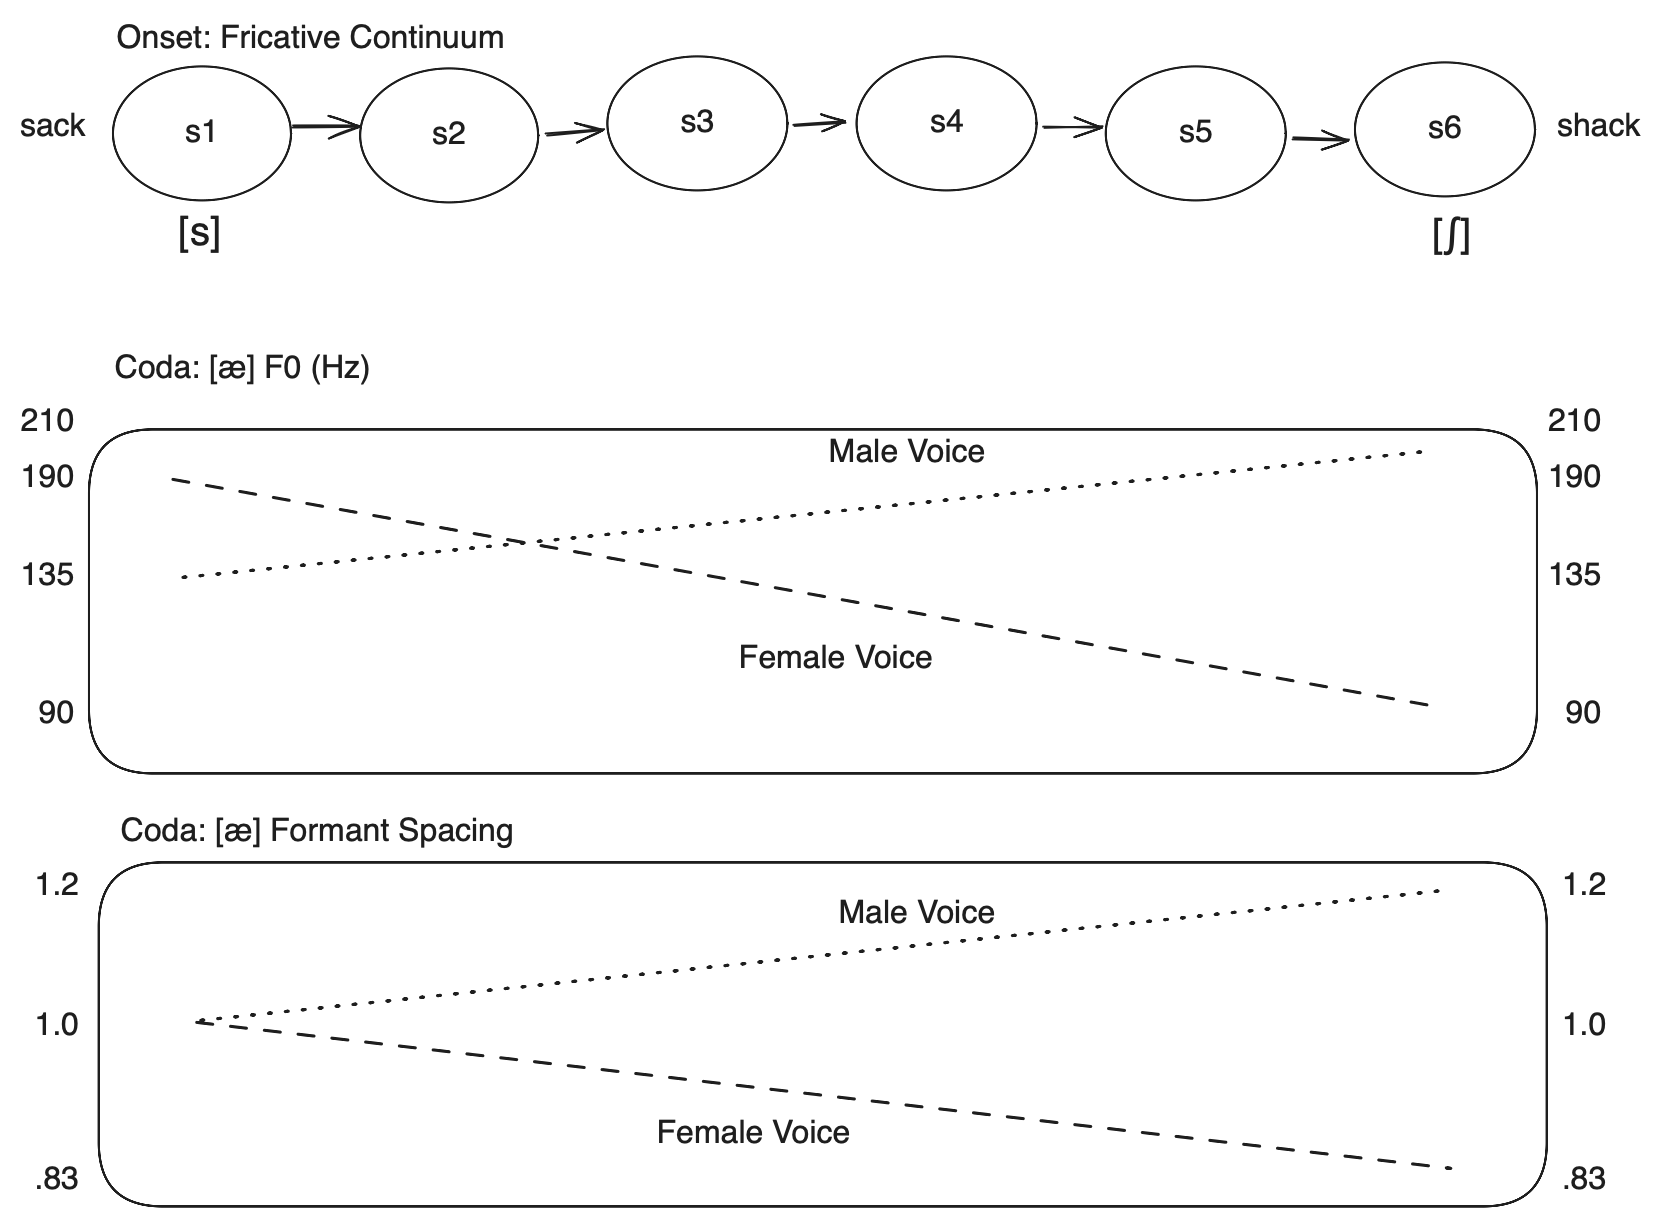
\includegraphics[width=0.8\linewidth,height=\textheight,keepaspectratio]{images/figure1.png}

}

\caption{\label{fig-stimuli}Bouavichith et al. (2019) auditory stimulus
continua. S1, S2, S3, S4, and S5 represent continuum steps from most
\emph{sack}-like to most \emph{shack}-like fricatives. F0 and F1:F2
Ratio plots show the manipulations to the Male and Female voiced
vowels.}

\end{figure}%

\subsection{Explicit Evaluations of Auditory
Stimuli}\label{explicit-evaluations-of-auditory-stimuli}

Because voices carry social information, we elicited explicit social
ratings to better understand how our auditory stimuli might influence
participants' perception of the identities of the two talkers.40
undergraduate students at the Ohio State University (25 female, 15 male,
ages 18-26) who participated in an in-person pilot version of the
inverse matched guise experiment were asked to make judgments regarding
the gender, gender prototypicality, and sexuality of a natural,
unresynthesized, production of \emph{sack} produced by each of the two
talkers. Participants listened to the recording and then selected from a
fixed set of responses; no free form responses were elicited.

Participants' judgments of the female voice indicate general agreement
about the gender identity of the speaker. Most participants (93\%)
indicated the speaker's gender to be female (2 participants further
specified `trans-female'), and 3 were unsure or otherwise unable to
determine the speaker's gender. For the female voice, average
prototypicality ratings (in which, for a given gender, 0 is least
prototypical, and 5 is most prototypical) were 4.3/5 if the participant
had indicated `female', and 2.75/5 if the participant had indicated
`trans female'. Judgements of the voice's sexuality were more variable,
with 54\% indicating they were unsure, 40\% indicating the speaker was
most likely heterosexual, and 1 participant each indicating the speaker
was most likely bisexual or another sexuality.

Participants' judgments of the male voice suggest similar agreement.
80\% of participants indicated the speaker's gender to be male,(1
further specified `trans-male') and 21\% were unsure of the gender of
the speaker. Average prototypicality ratings were lower for the male
speaker but similarly consistent: 3.6/5 if the participant had indicated
the voice belonged to a `male' speaker, and 2/5 if they had indicated
the person speaking was a `trans male'. As with the female voice,
judgements of the voice's sexuality were more variable. 65\% indicated
they were unsure, 14\% indicated the speaker was most likely
heterosexual, and 16\% indicated homosexual and, again, 1 each
indicating the speaker was most likely bisexual, or another sexuality
not listed. Crucially, no participants rated the female voice as male,
or the male voice as female. The variation among ratings may be due to
the presentation of options beyond binary female and male categories,
and/or to the current cultural understanding of gender performance as
distinct from sex. Despite this variability in responses, no
`implausible' answers were given. All things being equal, it is
reasonable for a listener to believe there may be little perceptual
difference in cis and trans voices for either male or female
performances Zimman (2018), and reasonable to consider `unsure' the most
acceptable option in lieu of asking the talker for their gender
identity.

\subsubsection{Visual Stimuli}\label{visual-stimuli}

The visual stimuli used in this study, again identical to the images
used in (Bouavichith et al. 2019), are shown in Figure~\ref{fig-visual}.
These included two face images, used for the guise manipulation, which
were retrieved from the Chicago Face Database (Ma, Correll, and
Wittenbrink 2015), a resource containing high-resolution, normed images
of faces indexed by gender and ethnicity. The faces selected were
normalized for both physical attributes (i.e., measurements of
particular facial dimensions), subjective ratings such as
attractiveness, and for gender and gender prototypicality. As in
Bouavichith et al., CFD-WF-015-006-N was selected as the representation
of the gender-protypical female talker and CFD-WM-029-023-N was selected
as the representation of the gender-prototypical male talker. Both
images were converted to greyscale at the command line using ImageMagick
(LLC 2023).

Additionally, two gray-scale line drawings were used as visual
representations of \emph{shack} and \emph{sack}. These images were used
in place of orthographic targets both to maintain consistency with
Bouavichith et al's design and to facilitate future eye tracking
investigation of this phenomenon.

\begin{figure}

\centering{

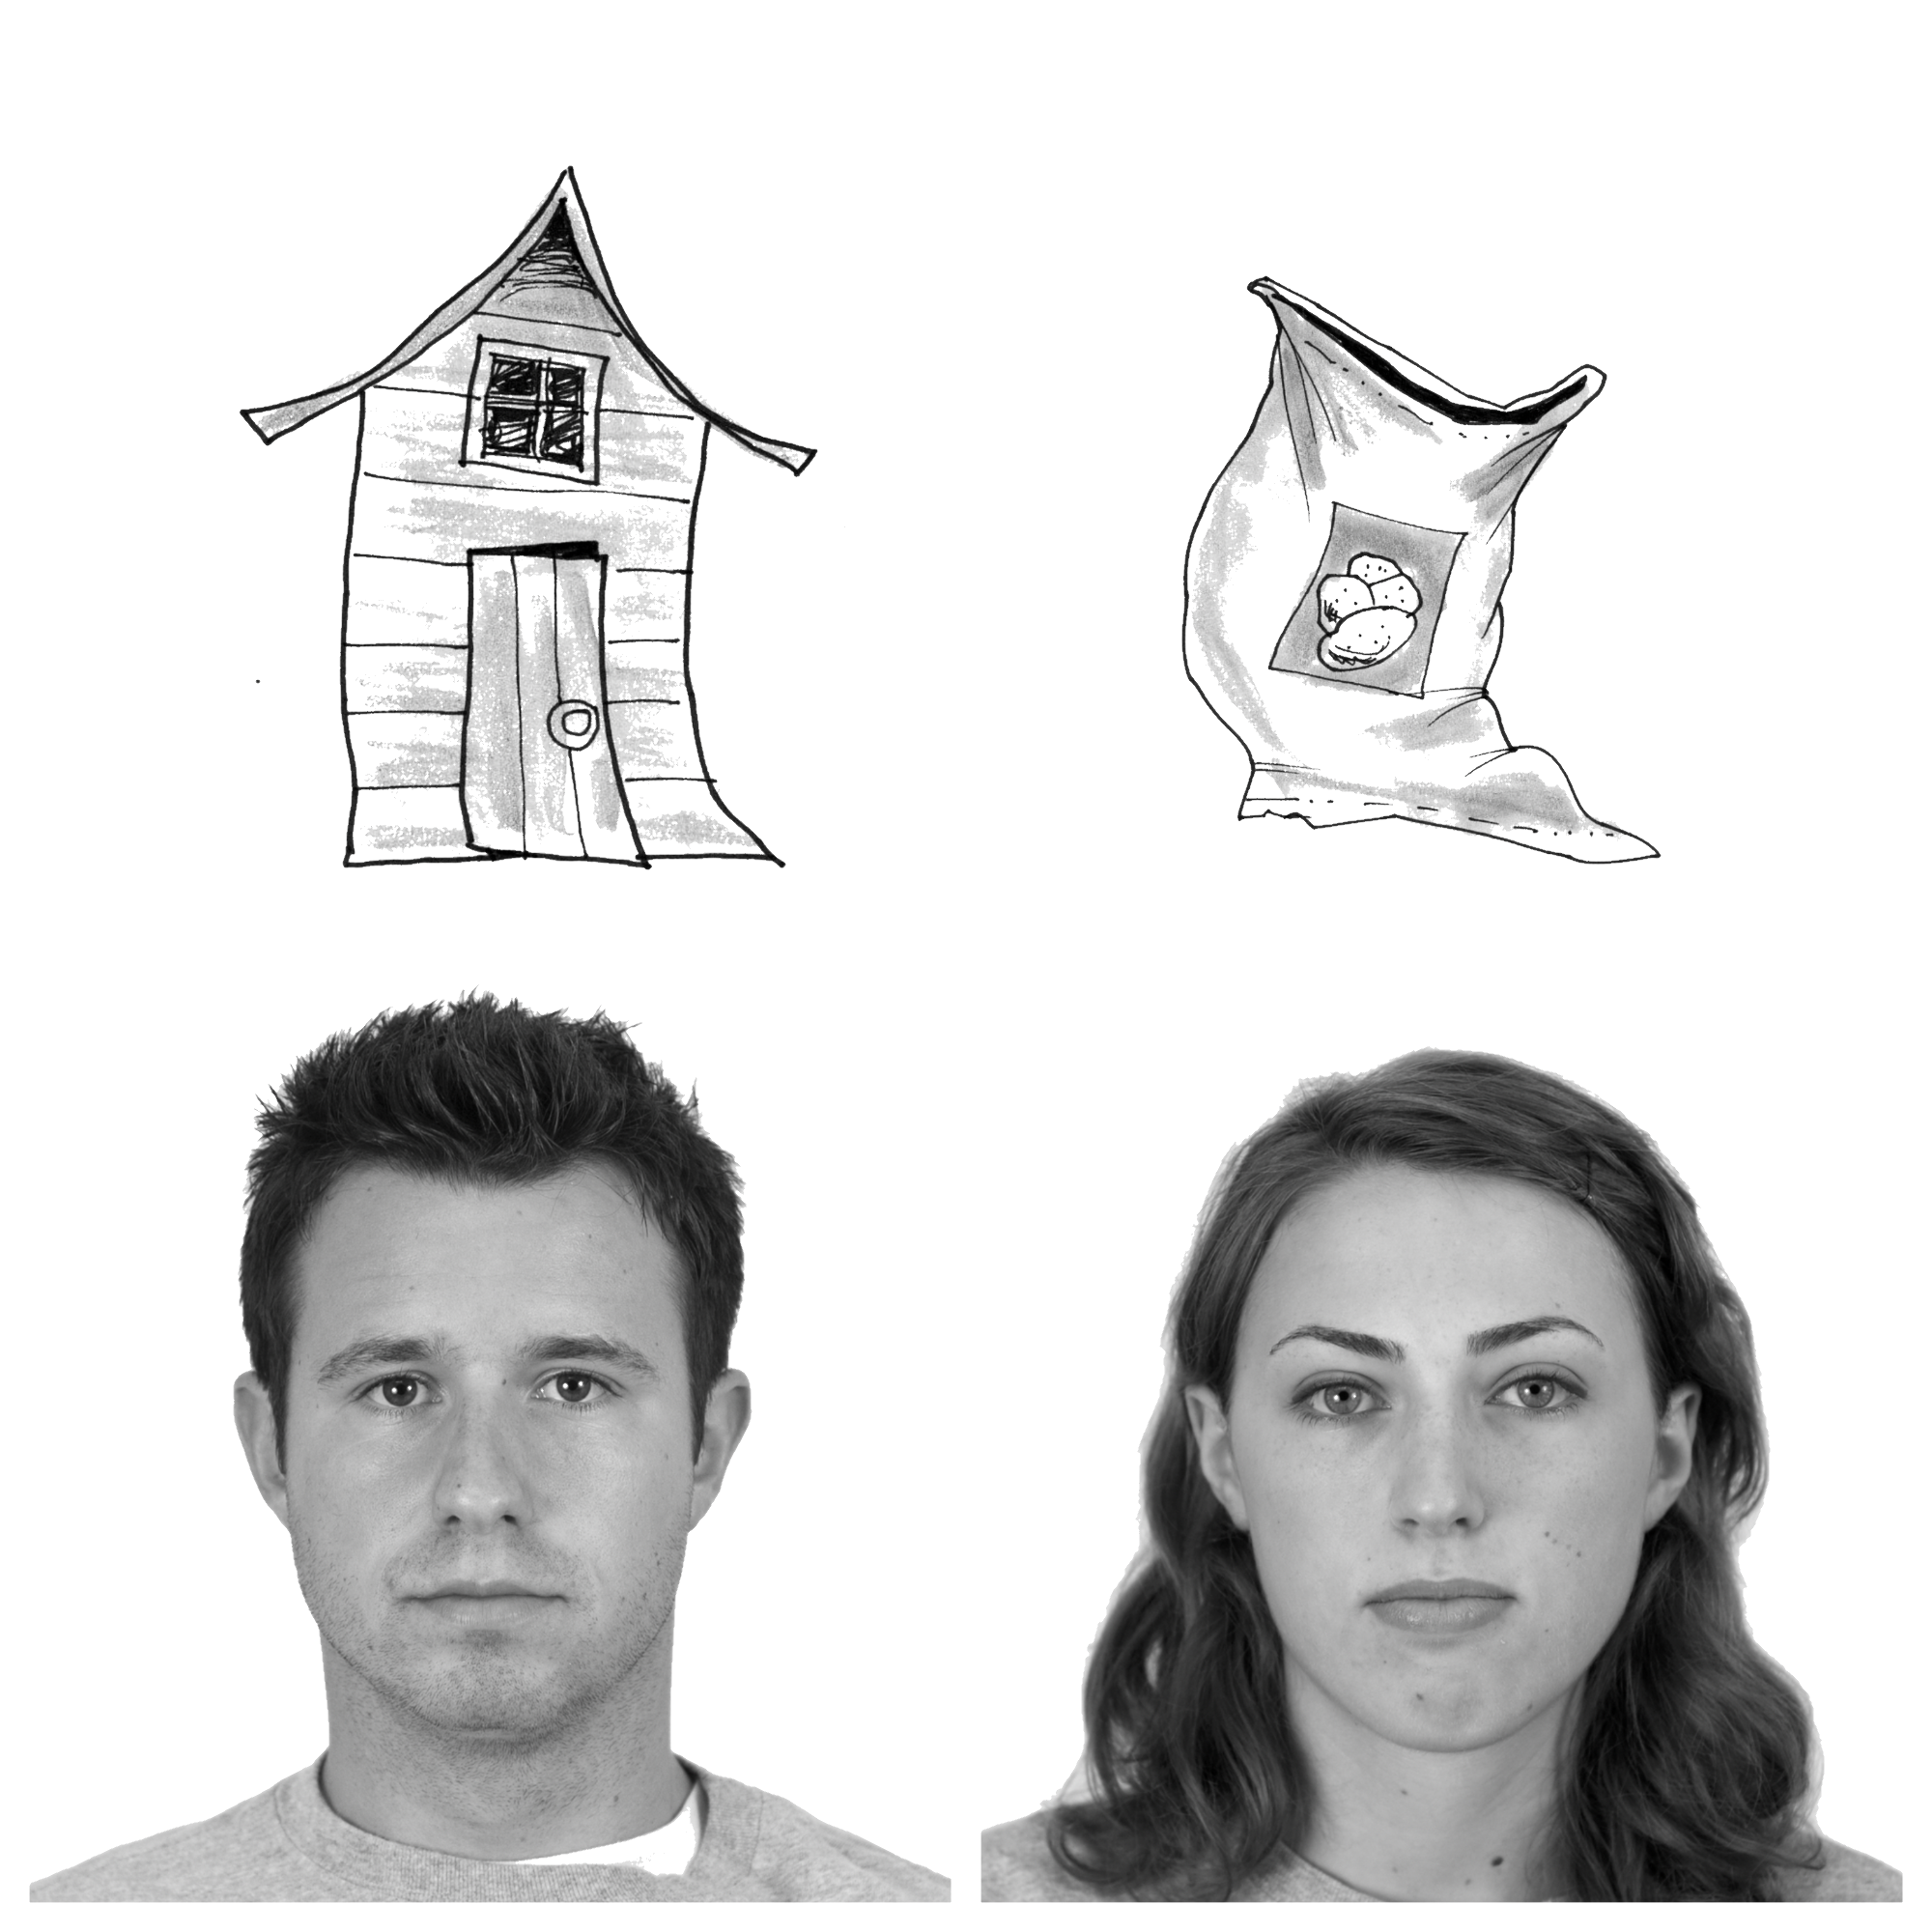
\includegraphics[width=0.8\linewidth,height=\textheight,keepaspectratio]{images/facesanddrawings.jpg}

}

\caption{\label{fig-visual}Stimuli comprised \emph{shack} and
\emph{sack} targets (top) and a gender-protypical `male' and `female'
face (bottom)}

\end{figure}%

\subsection{Procedure}\label{procedure}

The experiment was created in OpenSesame v3.3 (Mathôt, Schreij, and
Theeuwes 2012) and exported for the web using OSWeb v1.4.14.0.
Modifications to the experiment included translating portions of the
python code into JavaScript and adding code to collect Prolific IDs and
provide proof of completion to Prolific at the end of the experiment.
This experiment was hosted on a JATOS (Lange, Kuhn, and Filevich 2015)
instance hosted on an Ohio State University Linguistics Department
server. Participants received a link to the experiment via Prolific and
used their own computers, keyboards, and headphones to complete the
experiment.

In a between-subjects design, participants were randomly assigned to one
of two awareness conditions. These conditions differed only in the
initial information provided as to the nature of the experiment.
Participants in the \emph{hidden} condition experienced a standard
Matched Guise task. They were given no information about the task or the
stimulus materials beyond the general instructions for completing the
experiment: listen to the voice, press `z' if you heard the word on the
left, press `m' for the word on the right. Participants in the
\emph{unhidden} condition also received this instruction and were given
a partial debriefing regarding the task. They were informed that-- while
they would see faces onscreen while hearing words-- the voices in a
given trial were not produced by the person shown in the images, the
images had been downloaded from a database of photographs created at the
University of Chicago for experimental use, and that the auditory and
visual stimuli were in no way related to each other. Participants were
divided equally among these two conditions. Neither awareness condition
was informed about the synthetic nature of the auditory stimuli.

Additionally, participants were assigned to one of two gender congruity
conditions. Although the manipulated rimes sounded gender ambiguous to
us, and had been rated as ambiguous by (Bouavichith et al. 2019)'s pilot
participants, the possibility remained that the voices, particularly at
the end-points, might be perceived incongruously with the faces as in,
for example, (McGowan 2015)\footnote{We are choosing the words
  `congruous' and `incongruous' (Schulman 1974) intentionally to suggest
  faces and voices may pattern together in particular ways in listeners'
  experience and perception with no implied claim that voices may
  `match' or `mismatch' in some way that suggests either experimenters
  or participants have veridical access to an objective reality.}.

In congruous trials, the faces and voices were paired such that
participants were only presented with auditory stimuli from the female
talker's continuum alongside the female face and tokens from the male
talker were only presented alongside the male face. In incongruous
trials, by contrast, auditory stimuli from the female talker's continuum
were only ever presented alongside the male face and tokens from the
male talker's continuum were only ever presented alongside the female
face. Half of participants were randomly assigned to each congruity
condition, resulting in a 4-way between-subjects design across
instruction and congruity conditions. Each participant heard all 60
auditory stimuli; 30 paired with the male face and 30 paired with the
female face.

In each trial, participants were shown one of the two faces for 1500ms.
Following this initial presentation, the face remained onscreen and was
flanked by the \emph{shack} and \emph{sack} images. Simultaneously, one
of the auditory stimuli was played over the headphones. The trial ended
when the participant pressed an appropriate key on their physical
keyboard and their response and reaction time data were uploaded to the
JATOS instance. In both congruous and incongruous conditions, all 60
unique trials (30 per face) were presented twice to each participant for
a total of 120 trials.

\section{Predicted Results}\label{predicted-results}

\subsection{Face: male or female}\label{face-male-or-female}

Consistent with previous results, we expect to replicate the Strand
effect; in general, we anticipate that more of the {[}ʃ{]}-{[}s{]}
continuum will be heard as {[}ʃ{]} when participants are shown the
female face and more to be heard as {[}s{]} when participants are shown
the male face. However, these general predictions about the Face
presentation when the congruence of auditory and visual components of
the guise are taken as a whole.

\subsection{Congruence: pairing of face and
voice}\label{congruence-pairing-of-face-and-voice}

To our knowledge, the influence of congruence has not been directly
investigated for listeners' joint perception of gender and fricative
place. (Johnson, Strand, and D'Imperio 1999) tested AV integration of
Male and Female faces with prototypical and non-prototypical gendered
voices in a vowel quality perception task. They find what appears to be
an incongruence effect with the prototypical male voice; listeners
reported no difference in perceived vowel quality with this voice in
either Face condition (Johnson, Strand, and D'Imperio 1999, 376, Table
4). For this reason, we anticipate a replication of the Strand effect on
fricative identification in our congruous trials (when Face and Voice do
not conflict) but a failure to replicate for the incongruous trials
(when Face and Voice provide conflicting social information). This
difference may be stronger with the male voice, given both Johnson,
Strand, and D'Imperio's finding but also (King 2021).

We make a similar prediction for reaction times. (Johnson, Strand, and
D'Imperio 1999) did not collect reaction time data, but (McGowan 2011)
reports longer reaction times for incongruous trials, albeit in a very
different task, and (Whalen 1984) would seem to suggest that this should
hold for listeners' identification of fricatives on a {[}ʃ{]}-{[}s{]}
continuum. Specifically, we predict longer reaction times, in general,
for the Incongruous conditions. Furthermore, when gender information is
most clear, at gender continuum steps 1 and 2 for the Male talker and at
gender steps 4 \& 5 for the Female talker, and in conflict with the
presented Face, listeners' response times should be slower.

Since strong phonetic correlates of gender, F0 and F3, have been
manipulated over the course of the VC rime continua in our auditory
stimuli, we anticipate that the effect of incongruous face and voice
should be strongest for the natural end points of the continua where the
difference is most salient and weaker as phonetically-cued gender
information becomes more ambiguous. These stimuli have been
independently normed for ambiguity (Bouavichith et al. 2019, 1040, Table
1) in the 2nd and 3rd levels of the rime continua. This means we
anticipate an interaction between Face and Rime step but only in the
incongruous trials and only at the extremes of the rime continuum.

\subsection{Guise: Hidden or Unhidden}\label{guise-hidden-or-unhidden}

The primary goal of this experiment was to explore the role of listener
awareness and control in the matched guise technique. The tremendous
care researchers take to ensure that the guise manipulation is hidden
from participants suggests a kind of imagined fragility of the effects
of social information on language perception. From this view: listeners
who become aware of the guise manipulation will have introspective
access to and deliberative control over the influence of visual social
information on perception. If this is true, explaining the guise
manipulation, in the unhidden condition, should have a strongly negative
effect on the Strand effect. Alternatively, if the influence of social
information is not available to introspection or deliberative control,
we should see no change between the (traditional) hidden matched guise
and the unhidden guise.

Additionally, we speculate that there may be a response time difference
between the Hidden and Unhidden guises even if there is no apparent
difference in percept between the conditions. It can certainly be the
case that participants will arrive at the same behavioral responses via
different cognitive processing paths, perhaps drawing on different
levels of knowledge and awareness, and that these differences may be
visible in response times between the Instruction conditions.

\section{Results}\label{results}

Participants provided a total of 14,400 trials (120 trials from each of
120 online participants; 3600 trials in each instruction x congruity
condition). It is not clear what it means to be `accurate' when asked to
perceive fricatives from a continuum so accuracy was calculated only for
responses to the {[}ʃ{]} and {[}s{]} endpoints. Overall, participants
were highly accurate (96.8\%) but four participants were excluded from
further analysis for accuracy below the pre-determined 85\% threshold
reducing the total number of trials to 13,920. Trials were coded as
correct if the participant responded `shack' to onset step 1 or `sack'
to onset step 6. The four excluded participants all scored 67.5\%
accuracy or lower.

An additional 50 trials were excluded due to response times that were
either too fast or too slow. To reduce the effects of response time
outliers on subsequent analyses, all response times shorter than 50 ms
(N=0) and longer than 5000ms (N=50) were excluded. The 5000ms response
time cutoff was used instead of imposing an in-experiment time limit on
responses to a trial to ensure that participants were required to
respond to each trial. Altogether, 530 trials were excluded, leaving
data from 13,870 trials for analysis (approximately 96.3\% of the
initial data set). The majority (96.8\%) of the remaining response times
were within a range between 200 and 2000ms. To increase normality of the
distribution of response times across participants, the remaining
response times were log-transformed.

\subsection{{[}ʃ{]}-{[}s{]} Percepts}\label{ux283-s-percepts}

Figure~\ref{fig-scurve} presents listeners' percepts on this 2AFC task.
The horizontal axis in each of these four plots is the fricative
(syllable Onset) continuum step. Step 1 of the continuum is most
{[}ʃ{]}-like, step 6 is the most {[}s{]}-like, steps 3 \& 4 are the most
ambiguous. Darker lines in Figure~\ref{fig-scurve} present trials using
the female Face; lighter lines present trials using the male Face. The
Hidden and Unhidden instruction conditions are represented by the left
and right columns of figures, respectively. The rows present the
Congruous blocks where Face and Coda speaker voice shared a gender
identity (top) and Incongruous trials where Face and Coda speaker voice
mismatched in gender identity (bottom).

\begin{figure}

\centering{

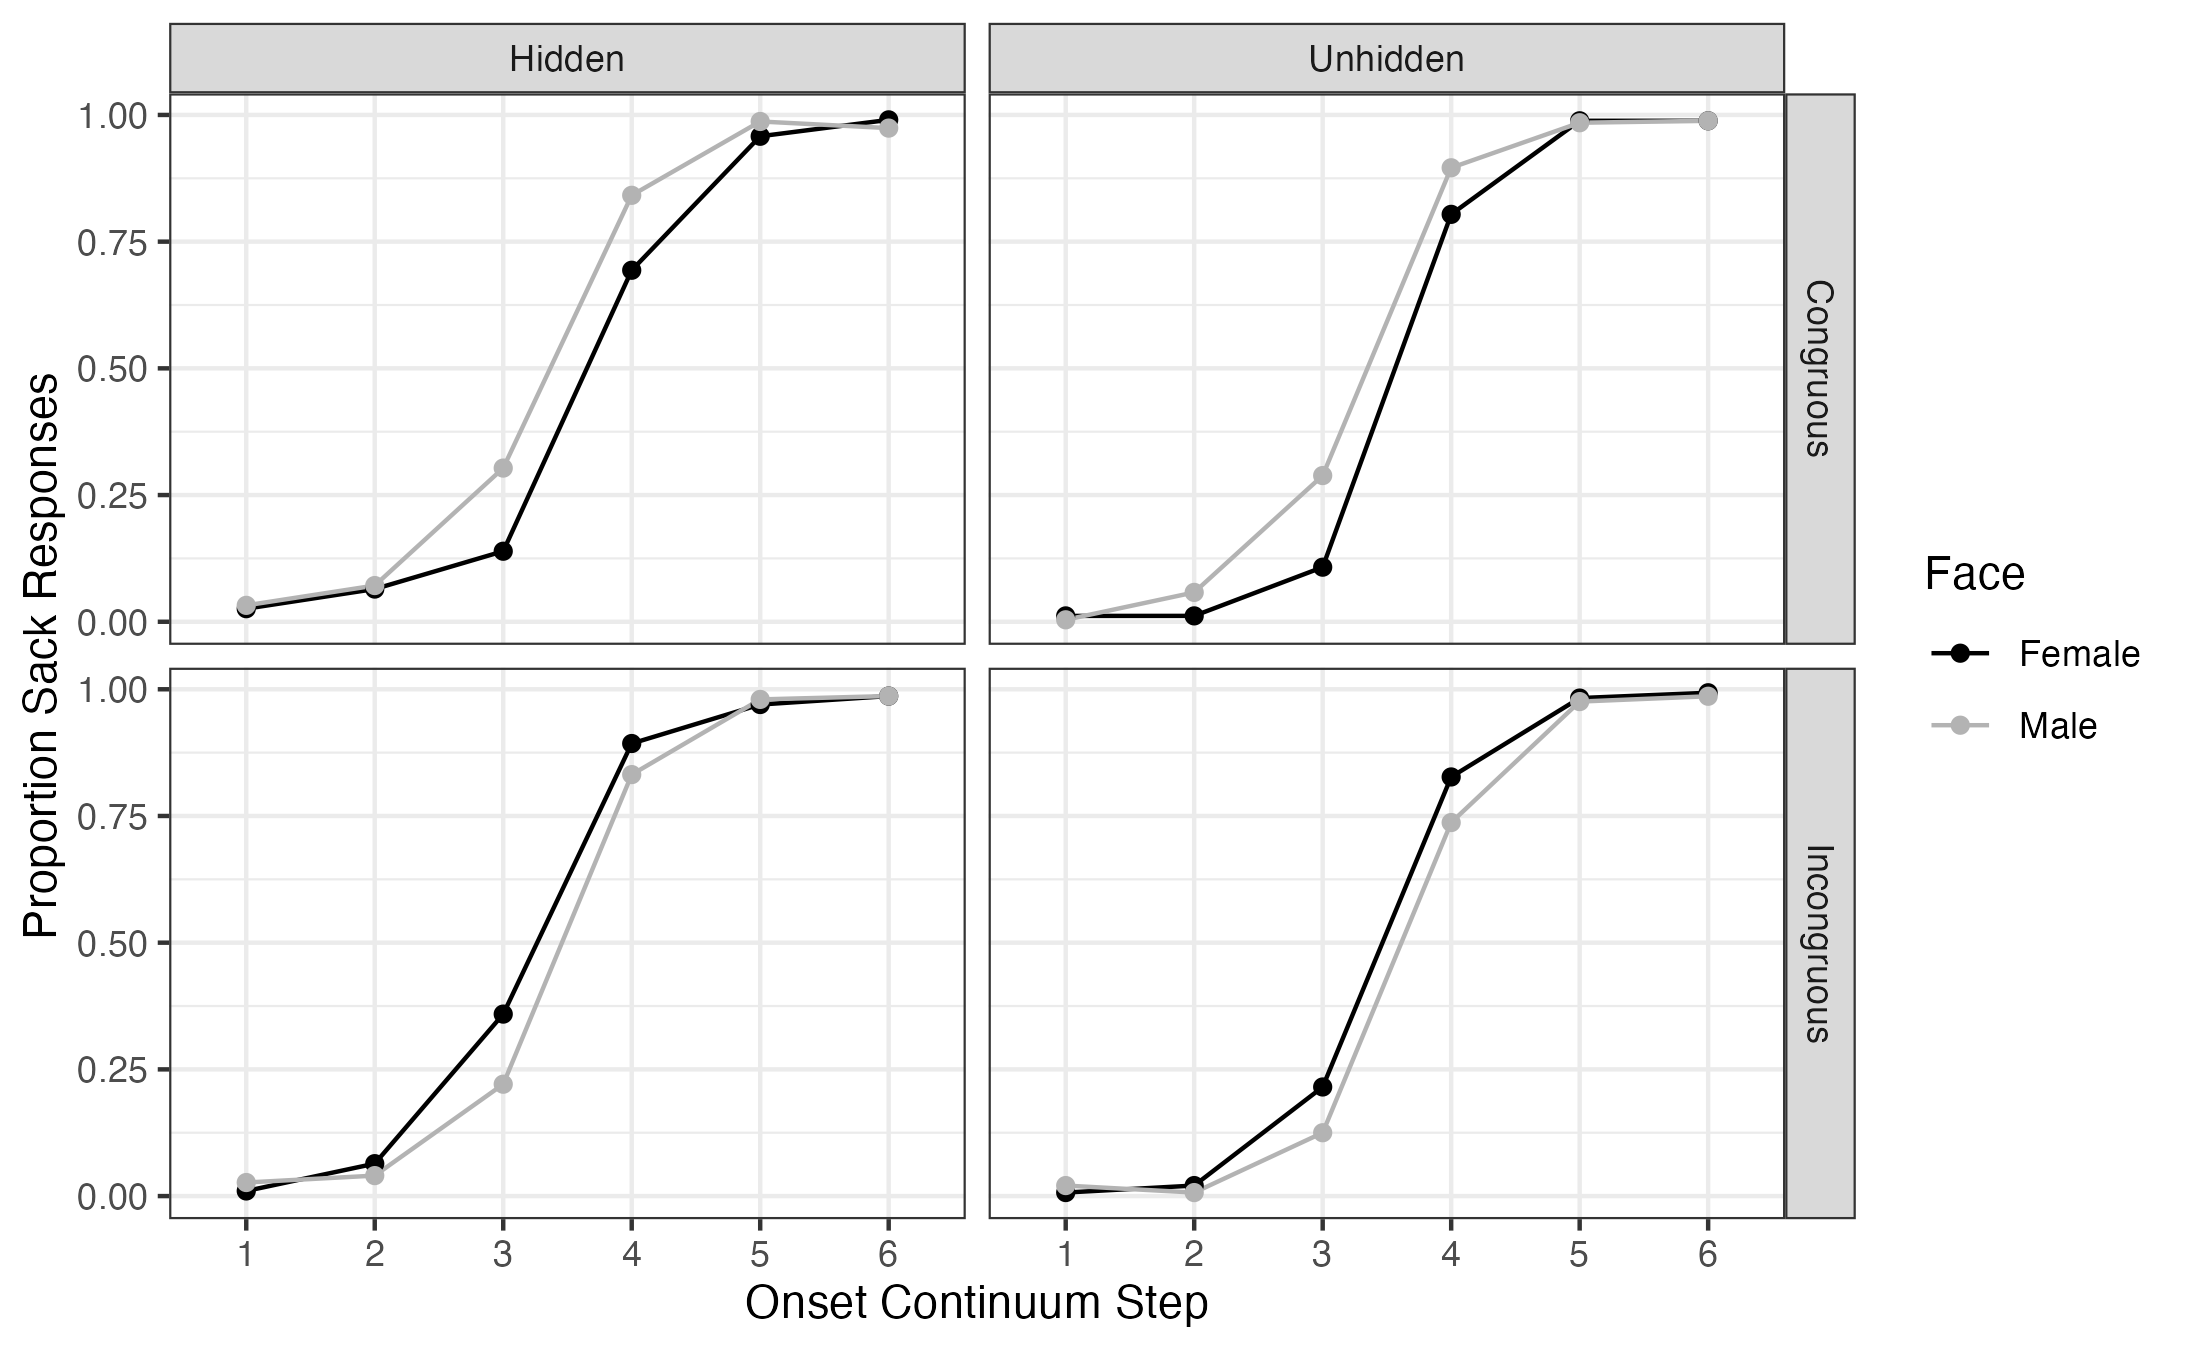
\includegraphics[width=0.8\linewidth,height=\textheight,keepaspectratio]{images/Scurve.png}

}

\caption{\label{fig-scurve}`sack' responses plotted as a function of
{[}ʃ{]}-{[}s{]} fricative (Onset) continuum steps and purported gender
presented by the face.}

\end{figure}%

A successful replication of the Strand effect would mean that a higher
proportion of the ambiguous stimuli would be heard as {[}s{]} when the
purported gender suggested by the face is male than when the face is
female. This pattern appears to hold in both the Hidden and Unhidden
conditions, but only when gender identity of the talker who produced the
CV rime stimuli was congruous with the gender presented in the visual
portion of the guise. From Figure~\ref{fig-scurve} it would appear that
listeners' reported percepts more closely track the voice of the talker
than the face in the picture when these sources of information are
incongruous.

\begin{figure}

\centering{

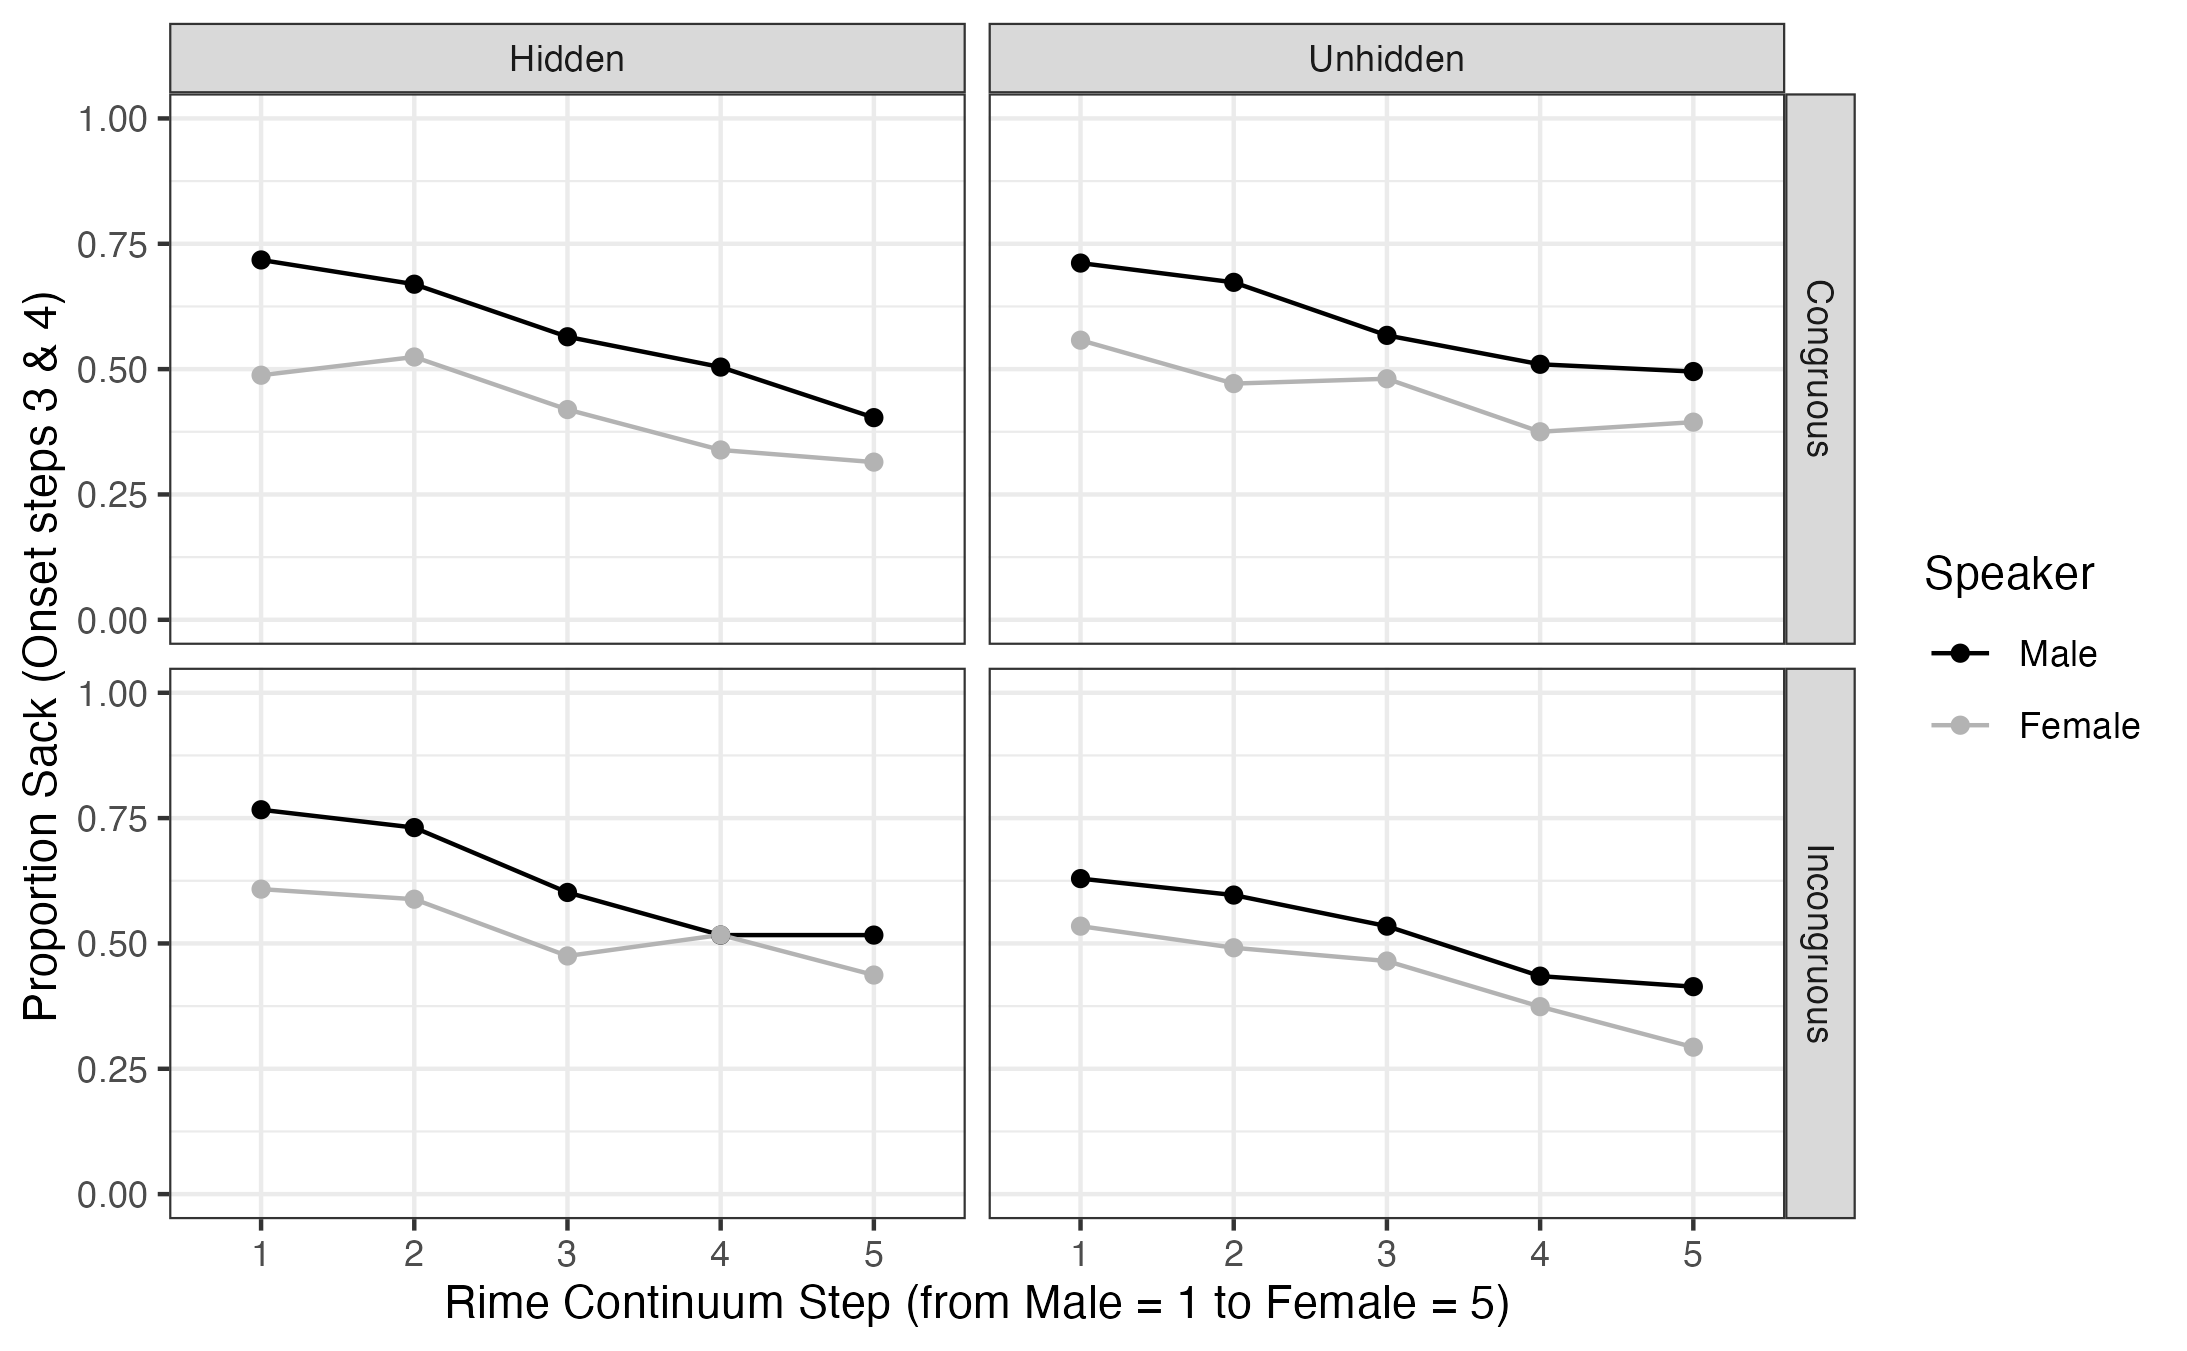
\includegraphics[width=0.8\linewidth,height=\textheight,keepaspectratio]{images/ambiguous-by-rime-step.png}

}

\caption{\label{fig-rimes}`sack' responses on ambiguous fricative trials
plotted as a function of CV rime continuum steps and gender identity of
stimulus talker.}

\end{figure}%

We predicted that, since strong phonetic correlates of gender have been
manipulated over the course of the VC rime continua, the effect of
incongruence should be strongest for the end points of the continua
where the social information presented by the voice is, presumably, most
salient and weaker as phonetically-cued gender information becomes more
ambiguous. Figure~\ref{fig-rimes} suggests that this prediction is at
least partially borne out. Figure~\ref{fig-rimes} plots proportion
`sack' responses to the ambiguous portion of the {[}ʃ{]}-{[}s{]}
continuum (steps 3 \& 4) as a function of rime continuum step. The
meaning of line color has changed in this figure. Dark lines represent
the male talker and lighter lines represent the female talker. Step 1 on
this continuum includes the most natural token for the male talker and
the most manipulated token for the female talker while step 5 includes
the most natural token for the male talker and the most manipulated
token for the female talker. As before, columns present the Hidden and
Unhidden conditions while rows present the Congruous and Incongruous
blocks.

In a 2AFC task with unbiased stimuli, chance is 50\%. Responses at the
.5 line in Figure~\ref{fig-rimes} suggest that the ambiguous fricatives
remained ambiguous while responses that tend to be above this line
reflect a tendency toward {[}s{]} percepts and responses that tend to be
below this line reflect a tendency toward {[}ʃ{]}. Across all 4
conditions we observe a declination from highest-proportion {[}s{]}
responses in step 1 of the F0 continua to lowest in step 5. When face
and voice were congruous, virtually all male-voice (and male face)
responses are above or at 50\% `sack' and virtually all female-voiced
(and female face) responses are at or \emph{below} 50\% `sack'. This is
the same pattern that can be observed at Onset continuum steps 3 \& 4 in
Figure~\ref{fig-scurve}. It is not clear from Figure~\ref{fig-rimes}
alone if there is any difference at all between the Congruous and
Incongruous conditions. However, it is important to recall about the
bottom row of this figure that male talker responses in the incongruous
trials were presented with a female face while female talker trials were
presented with a male face. Even a weakly-significant Strand effect
would predict that the female talker, particularly on the more ambiguous
continuum steps, should show more `sack' responses consistent with
having been shown a male face and no such effect is evident in this
plot.

Indeed, a striking feature of these figures
(\ref{fig-scurve}, \ref{fig-rimes}) is how the apparent influence of
gender information flips between congruous and incongruous conditions in
the former but remains essentially constant in the latter. Taken
together, these plots suggest that cues to gender in F0 is a stronger
predictor of listeners' reported percept in this matched guise task than
just the purported gender of the face.

Finally, the main objective of this experiment was to explore the role
of listener awareness in the matched guise technique. Here again there
may be differences between the congruous and incongruous conditions that
will be better understood through quantitative analysis, but the overall
trend is clear. If there is an effect of explaining to participants that
the voice and face in the matched guise task are unrelated to each
other, that effect is so weak as to be essentially invisible in these
visual interrogations of the data. Categorical responses in the Hidden
and Unhidden instruction conditions appear to be identical.

\subsection{Logistic Regression and Quantitative
Analysis}\label{logistic-regression-and-quantitative-analysis}

These qualitative assessments of listener responses can be examined
further through quantitative analysis. Through model comparison we
initially arrived at a logistic mixed model to predict percept with
Congruity condition, instruction condition, Onset step, Face, and Rime
step with interactions for all but Rime step. This model was justified
by model selection but given the notorious difficulty of interpreting a
4-way interaction and the preceding visual interrogation of the data, we
opted to separate Congruence into a pair of 3-way models. Using
\texttt{glmer()} (Bates, Maechler, and Bolker 2011), we divided the data
into congruous and incongruous subsets and fitted a pair of logistic
mixed models (estimated using ML and BOBYQA optimizer) to predict
percept with Instruction condition, Onset.step, Face and Rime step
(\texttt{percept\ \textasciitilde{}\ Instruction\ *\ Onset.step\ *\ Face\ +\ Rime.step}).
The models included random intercepts for subject. All categorical
predictors were coded using contrast coding.

\begin{figure}

\centering{

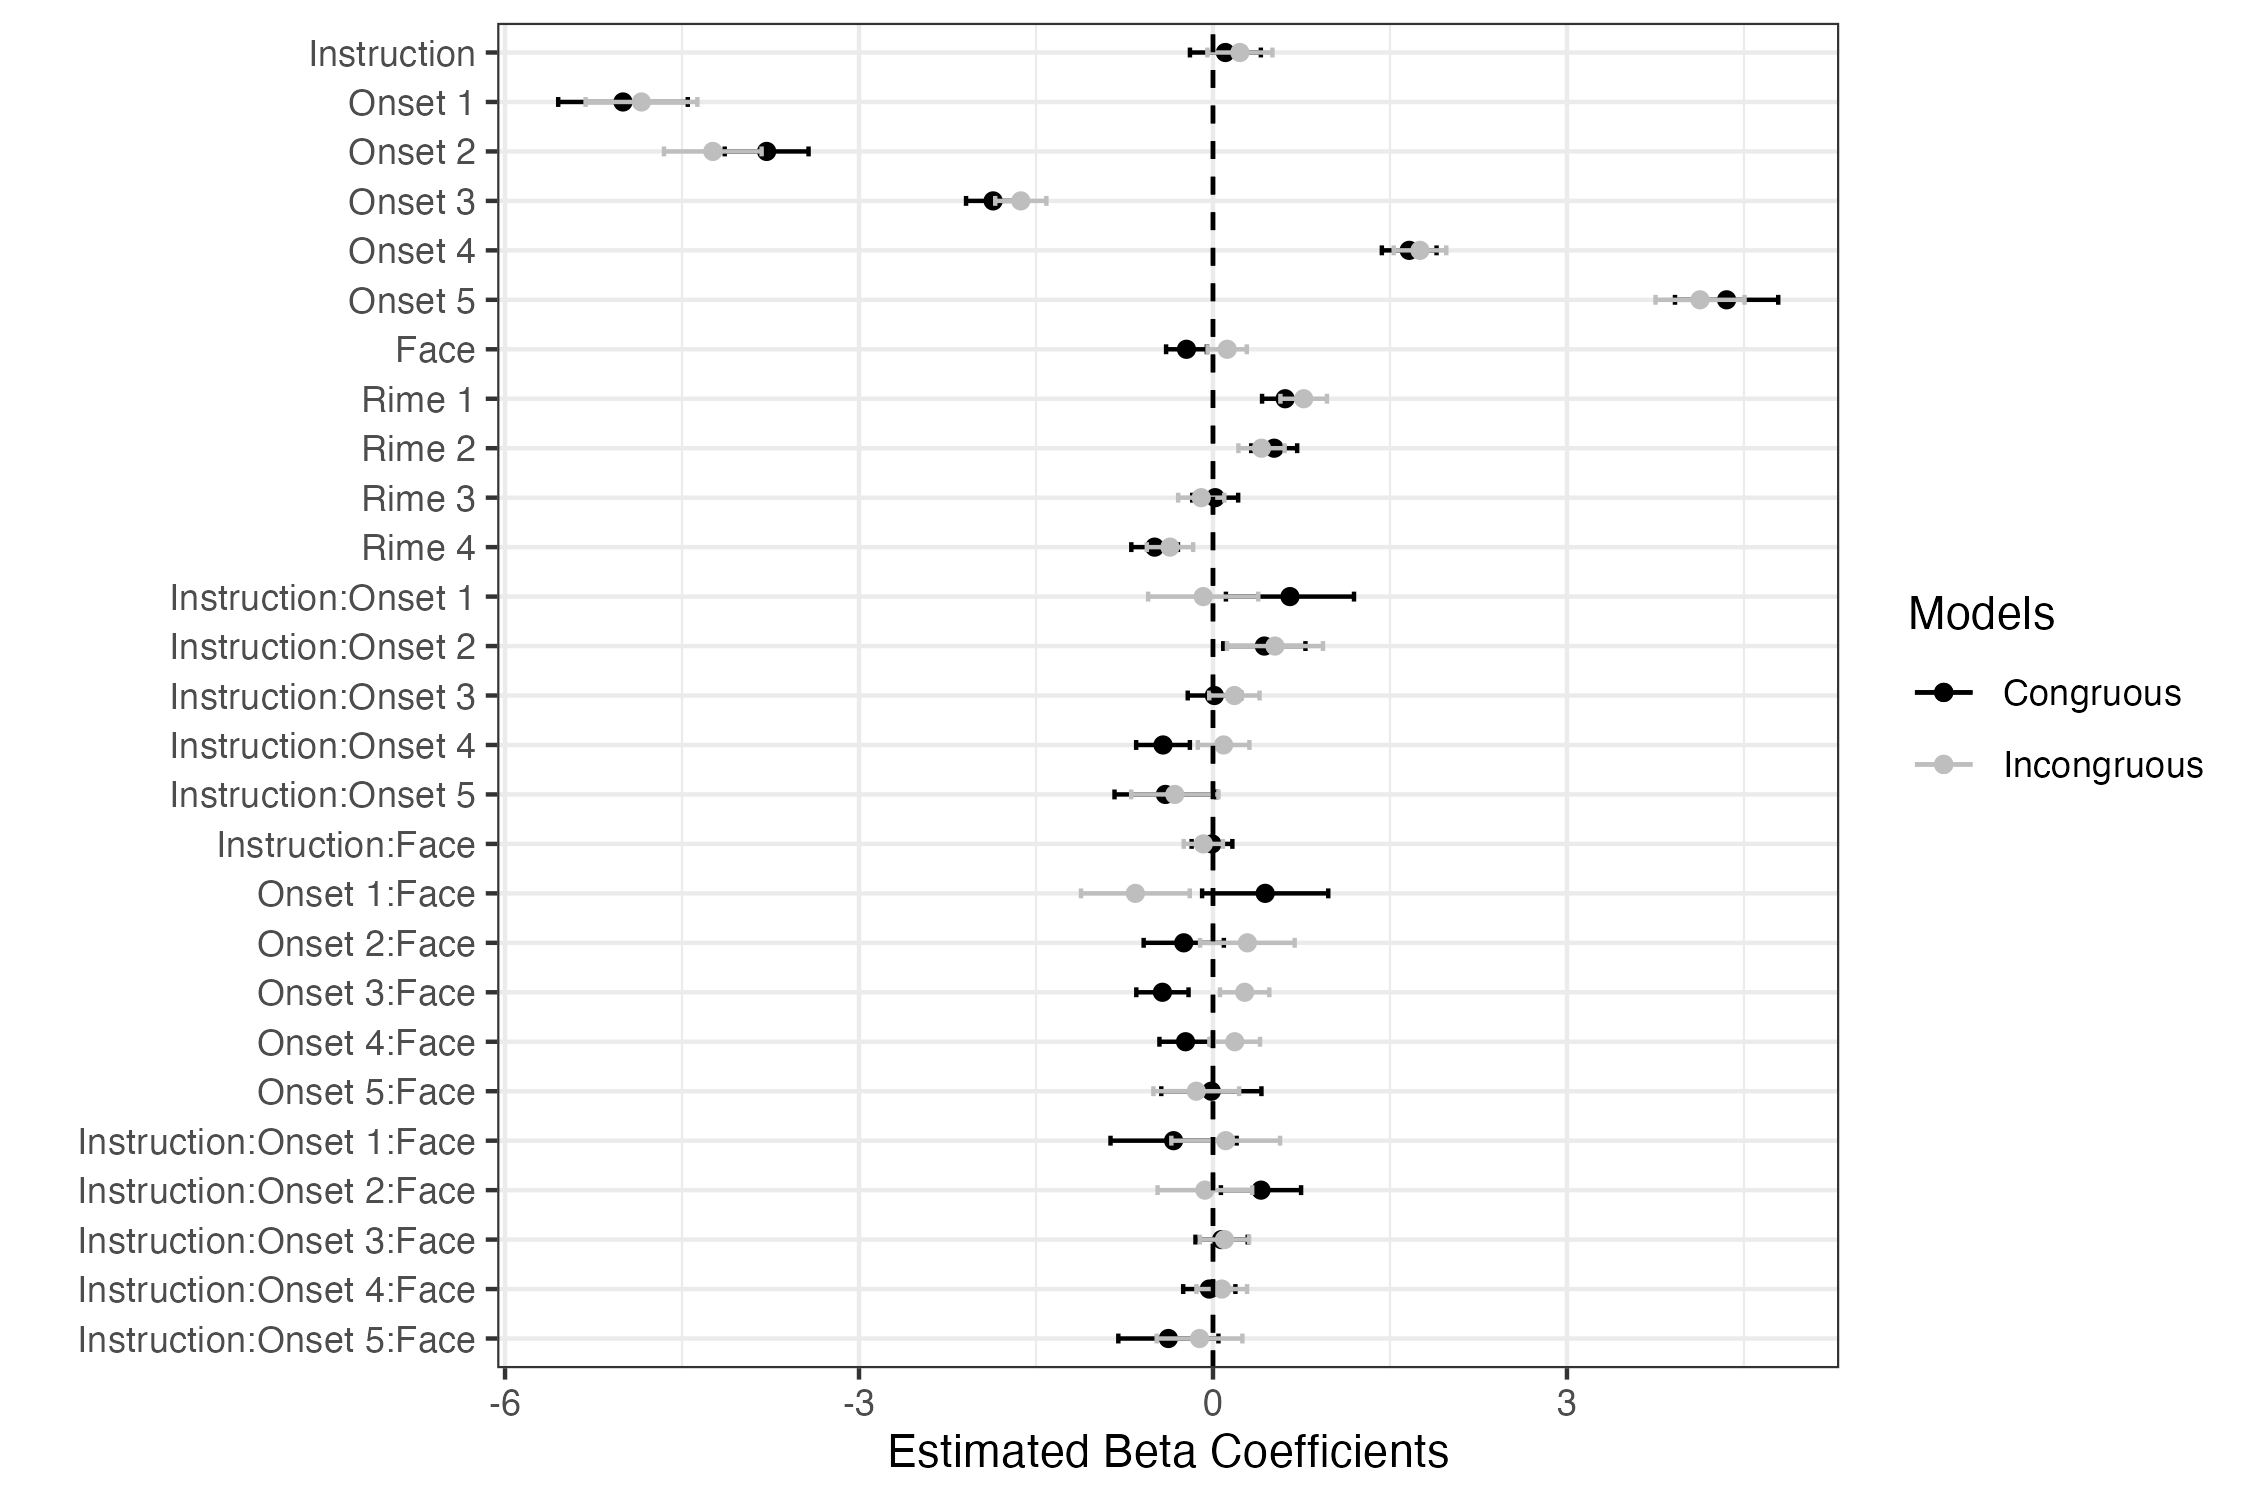
\includegraphics[width=0.8\linewidth,height=\textheight,keepaspectratio]{images/coefs_instruction.png}

}

\caption{\label{fig-coefs}Beta coefficients for listener responses in
the Congruous (black) and Incongruous (gray) logistic regression models
plotted with 95\% confidence intervals.}

\end{figure}%

Beta coefficients for the two separate logistic mixed models are plotted
together in Figure~\ref{fig-coefs}. Terms plotted to the left of the
dashed zero line have a negative influence on `sack' percepts in the
model while terms plotted to the right have a positive influence. As a
consistency check we can observe that the levels of the Onset continuum
behave in precisely the expected ways and all levels are statistically
significant predictors of percept in both models. Onset step 1 ({[}ʃ{]})
is negatively associated with `sack' responses and significant in both
the Congruous (\(β=-5.00\), \(SE=0.28\), \(p < 0.001\)) and Incongruous
(\(β=-4.84\), \(SE=0.24\), \(p < 0.001\)) models. Onset step 5 ({[}s{]})
is positively associated with `sack' responses and significant in both
the Congruous (\(β=4.35\), \(SE=0.22\), \(p < 0.001\)) and Incongruous
(\(β=4.12\), \(SE=0.19\), \(p < 0.001\)) models.

As visual inspection of the data suggests, this study includes a
replication of the Strand effect in the Congruous condition. There is a
main effect of Face in the model (\(β=-0.22, SE=0.09, p<0.05\)). Face is
negatively associated with `sack' responses suggesting that, with these
stimuli, at least, it is more appropriate to understand the effect of
Face as an increase of `shack' responses given the female Face. The
inclusion of the interaction term for Onset and Face allows us to see
that the effect of Face is greatest on the ambiguous Onset steps 3
(\(β=-0.43\), \(SE=0.11\), \(p < 0.001\)) and, to a lesser extent, 4
(\(β=-0.23\), \(SE=0.11\), \(p < 0.05\)).

However, the Strand effect observed in the Congruous condition is not
attributable entirely to the main effect of Face. Rime F0 is also
significant; Rime level 1, the male end of the continuum, is positively
associated with `sack' responses (\(β=0.61\), \(SE=0.10\),
\(p < 0.001\)) as is Rime level 2 (\(β=0.52\), \(SE=0.10\),
\(p < 0.001\)). Rime level 3, where the continuum is most gender
ambiguous, is not statistically significant. Rime level 4, on the female
end of the continuum, is negatively associated with `sack' responses and
significant (\(β=-0.49\), \(SE=0.10\), \(p < 0.001\)).

Unsurprisingly, the Strand effect has not been replicated in the
incongruous condition. As is visible in the bottom row of
Figure~\ref{fig-scurve}, the effect of Face on `sack' responses is not
significant. The interaction of Onset and Face also behaves quite
differently in the Incongruous model. Onset x Face is negatively
associated with `sack' responses at Onset step 1 (\(β=-0.66\),
\(SE=0.24\), \(p < 0.001\)) but positively associated with `sack'
responses and significant at Onset step 3 (\(β=0.27\), \(SE=0.11\),
\(p < 0.05\)).

Interestingly, the significant effect of Rime observed in the Congruous
model also holds, nearly identically, in the Incongruous model. Rime
level 1, the male end of the continuum, is again positively associated
with `sack' responses (\(β=0.77\), \(SE=0.10\), \(p < 0.001\)) as is
Rime level 2 (\(β=0.41\), \(SE=0.10\), \(p < 0.001\)). Rime level 3 is
also not statistically significant in the Incongruous model. Rime level
4, on the female end of the continuum, is negatively associated with
`sack' responses and significant (\(β=-0.36\), \(SE=0.10\),
\(p < 0.001\)).

Finally, the quantitative analysis of the primary objective of this
experiment, exploring the effect of unhiding the matched guise
manipulation from participants, largely supports the qualitative
analysis. As can be observed in Figure~\ref{fig-coefs}, there is no
significant main effect of Instruction condition in either model. Still,
a somewhat more nuanced picture emerges from the interactions of
Instruction condition with Onset and the 3 way interaction of
Instruction, Onset, and Face in the Congruous trials. The interaction of
Instruction with Onset is significant, or nearly so, at every step of
the fricative continuum other than the most significant. In the
{[}ʃ{]}-like portion of the continuum, the interaction with face is
positively associated with `sack' responses at step 1 (\(β=0.65\),
\(SE=0.28\), \(p < 0.05\)) and 2 (\(β=0.44\), \(SE=0.18\),
\(p < 0.05\)). The interaction of guise with the most ambiguous onset
step is not significant (\(β=0.011\), \(SE=0.12\)). The interaction of
Instruction with Onset step 4, on the {[}s{]} end of the continuum is
negatively associated with `sack' responses and statistically
significant (\(β=-0.43\), \(SE=0.12\), \(p < 0.001\)). Instruction x
Onset step4 is also negatively associated with `sack' responses but does
not reach significance at the standard alpha level (\(β=-0.40\),
\(SE=0.22\), \(p = 0.067\)). The 3-way interaction of Instruction x
Onset x Face is positively associated with `sack' responses at step 2
(\(β=0.41\), \(SE=0.17\), \(p < 0.05\)) and weakly, but not
significantly, negatively associated with `sack' responses at step 5
(\(β=-0.38\), \(SE=0.21\), \(p = 0.080\)).

There is also no main effect of Instruction in the Incongruous trials.
The 3-way interaction of Instruction x Onset x Face, while justified by
model selection for inclusion in this model, also does not reach
statistical significance. However the 2-way interaction of Instruction
with Onset step is positively associated with `sack' responses at Onset
step 2 (\(β=0.53\), \(SE=0.21\), \(p < 0.05\)) and approaches
significance at step 3, where it is weakly positively associated
(\(β=0.18\), \$SE=0.11, \(p = 0.095\)) and step 5 where it is weakly
negatively associated (\(β=-0.32\), \(SE=0.19\), \(p = 0.086\)).

\subsection{Response Times}\label{response-times}

As with the logistic regression models, we again opted to separate
Congruence into a pair of 3-way models for linear mixed model analysis
of our log-transformed response time data. Using \texttt{lmer()} (Bates,
Maechler, and Bolker 2011), we reused the congruous and incongruous
subsets created for the logistic regression models and We fitted a
linear mixed model (estimated using REML and nloptwrap optimizer) to
predict logRT with Guise, Onset, Face and Rime
(\texttt{logRT\ \textasciitilde{}\ Instruction\ *\ Onset\ *\ Face\ +\ Rime}).
The models included random intercepts for subject. All categorical
predictors were coded using contrast coding. Beta coefficients for both
models are plotted in Figure~\ref{fig-coefs-logRT}. Terms plotted to the
left of the zero line are associated with a decrease in log response
time while terms plotted to the right of the zero line are associated
with an increase in log response time. Notably, the longest response
times are associated with the most ambiguous steps of the
{[}ʃ{]}-{[}s{]} onset continuum. Onset step 3 is positively associated
with response time and significant in both the congruous (\(β=0.08\),
\(SE=0.007\), \(p < 0.001\)) and incongruous (\$β=0.0\$7, \(SE=0.007\),
\(p < 0.001\) ) models. The same is true of step 4 in the congruous
(\(β=0.07\), \(SE=0.007\), \(p < 0.001\)) and incongruous (\(β=0.07\),
\(SE=0.007\), \(p < 0.001\)) models as well. On the other hand, steps 1,
2, and 5 are all negatively associated with response time and also
significant in both models (see Figure~\ref{fig-coefs-logRT}).

\begin{figure}

\centering{

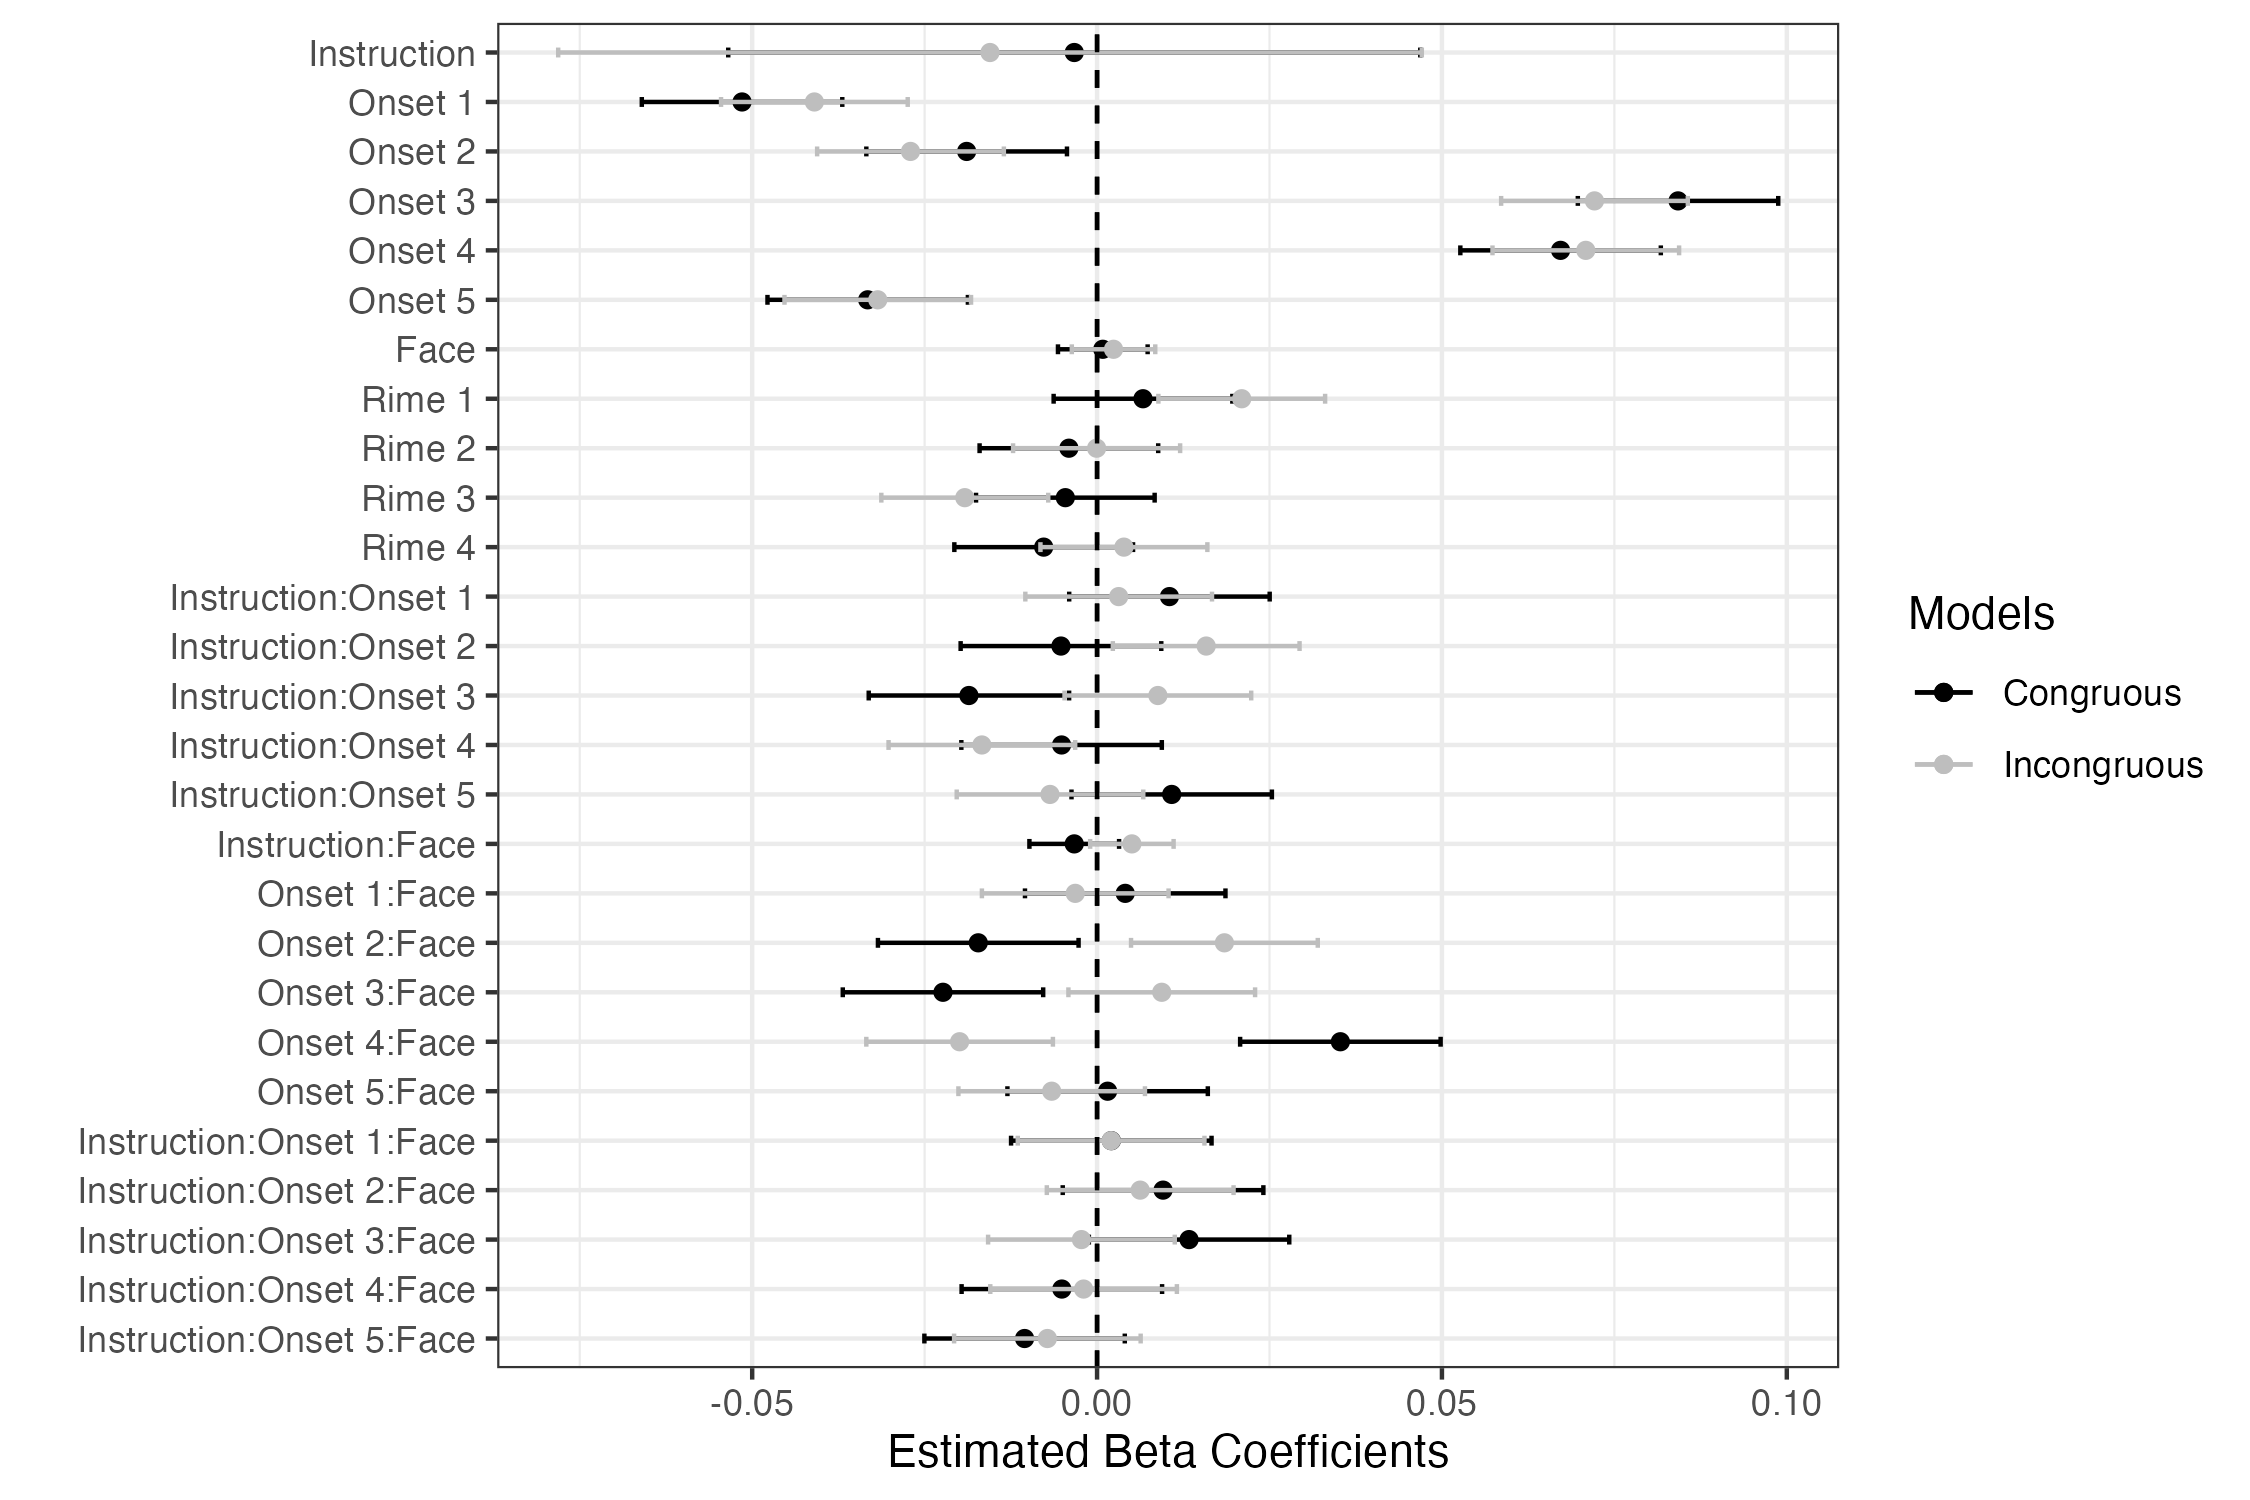
\includegraphics[width=0.8\linewidth,height=\textheight,keepaspectratio]{images/coefs-logRT_instructions.png}

}

\caption{\label{fig-coefs-logRT}Beta coefficients for log-transformed
response times in the Congruous (black) and Incongruous (gray) linear
regression models plotted with 95\% confidence intervals.}

\end{figure}%

We predicted overall slower response times in the Incongruous than
Congruous conditions and this prediction is not borne out by the data.
Apart from generally higher variability in the incongruous conditions,
there is no positive or negative trend in response times between the two
Congruity models. For example, within the Incongruous model response
times given the interaction of Onset step 3 * Face are longer
(\(β=-0.009\), \(SE=0.007\), \(p = 0.17\)), which would seem to support
our prediction, but response times for Onset step 4 * Face are shorter
(\(β-0.02\), \(SE=0.007\), \(p < 0.01\)), the opposite of what we
predicted. The exact opposite pattern appears within the Congruous model
where response times are shorter given Onset 3 * Face (\(β=-0.02\),
\(SE=0.007\), \(p < 0.01\)) but longer given Onset step 4 * Face
(\(β=0.04\), \(SE=0.007\), \(p < 0.001\)). These crossing patterns can
be seen in Figure~\ref{fig-coefs-logRT}.

Given the replication of the Strand effect in the Congruous, but not the
Incongruous conditions described in the previous section, it may be
notable that there is a significant main effect of Face in the Congruous
model where it is negatively associated with response time (\(β=0.22\),
\(SE=0.08\), \(p < 0.05\)) and not significant in the Incongruous model.

\section{Discussion}\label{discussion}

The question that motivated this study was a desire to understand the
role of listener awareness and control in the matched guise technique.
We believe that the careful measures researchers generally employ to
obscure the nature of the guise manipulation from participants is
attributable to a long-held assumption in the sociolinguistics
literature that social knowledge is high-level knowledge, available to
introspective control, and that this differs from linguistic knowledge
which is low-level knowledge, unavailable to control (Campbell-Kibler
2016). The results of the present study are inconsistent with this
imagined fragility of the influence of social knowledge. Revealing the
nature of the guise manipulation did not significantly influence
listener responses in either the congruous or incongruous conditions.
Nor did this revelation have a significant influence on response times
in either condition.

The finding that the Matched Guise effect holds for speech perception
both when hidden from the participant and when unhidden is inconsistent
with a model of processing in which social knowledge simply acts as a
filter on linguistic knowledge. Social knowledge influences perception
even when listeners are aware that it is, or may be, false. This result
parallels previous results for accentedness and attractiveness judgments
(Campbell-Kibler 2021). A similar result may be present, for social
information, in the within-participants guise manipulation of (McGowan
and Babel 2020). In that study, the authors use participants'
metalinguistic commentaries to assess the extent to which the guise
manipulations were or were not `believed'. The results of the present
study suggests that that belief may be irrelevant. The present result
also gives additional context to studies demonstrating influence of
social knowledge even when listeners have no reason to believe the guise
manipulation (Niedzielski 1999; Hay, Nolan, and Drager 2006; Hay and
Drager 2010). It is unclear whether social knowledge will prove to be as
resilient to awareness as the obligatory McGurk effect (McGurk and
MacDonald 1976) which persists even when participants actively identify
that the face and voice in the experiment are mismatched (Green et al.
1991b), but the suggestion is that it will.

The gender identity of the talker who produced the VC Rime supplemented
Face in the Congruous conditions to make the Strand effect even
stronger; the mechanism may prove similar to the way lip-rounding
accentuates the backness of back vowels. In the Incongruous conditions,
though, listeners' perception of the {[}ʃ{]}-{[}s{]} continuum tracked
the VC Rimes, rather than the purported gender of the Face. This pattern
was strongest in the least-ambiguous portions of the Rime continuum and
weakest in the most-ambiguous. In a sense, by separating trials by
congruity of face and voice we have replicated (Strand and Johnson
1996)'s exp1 and exp2 simultaneously. One wonders, looking back at their
exp2, whether this classic result was \emph{also} a congruous condition
in which listeners had sufficient gender information from the voice to
supplement the purported information from the Face. Even the
non-prototypical voices used in that study did pattern, in exp1, in
weakly gendered ways. This finding may provide some insight into recent
failures to replicate the original Strand effect (Schellinger, Munson,
and Edwards 2017; Wilbanks 2022).

The phonetic correlates of gender manipulated in the VC rimes for this
study are F0 and formant ratios. However, these may not be the only cues
listeners are drawing upon with their knowledge of US English. Surely,
F0 and vowel formant ratios \emph{can be} important to listeners, just
as voice onset time and vocal fold vibration can be important cues to
the voicing of /t/ and /d/. But as (Lisker 1986) catalogs, there are 16
cues to this apparently simple feature in English, any of which might be
sufficient to communicate voicing, but none of which is required. In
this study we have used manipulated stimuli that obscure, over the
course of two gender continua, the gender identity of the talker who
produced the basis token for that continuum. At an explicit level, these
continua \emph{sound ambiguous} to the experimenters in much the way
that (Whalen 1984)'s stimuli do not sound obviously mismatched. But our
perception results suggest that listeners are still aware, albeit
implicitly, of the gender identity we have attempted to obscure by
altering the phonetic correlates of gender.

\section{Conclusion}\label{conclusion}

Decades of research since (Strand and Johnson 1996)`s original finding
have demonstrated that a visual cue can shift fricative perceptions when
paired with an ambiguously-gendered voice (although cf Munson 2017 and
Wilbanks 2022). (Bouavichith et al. 2019) demonstrated with eye-tracking
that this effect is fast and bi-directional. One could come away from
Strand \& Johnson's exp1 and exp2 and subsequent replications with a
theoretical model in which visually-cued social information and
phonetically-cued social information exert equivalent influence on
speech perception. Prototypically-gendered voices can shift perception
of a {[}ʃ{]}-{[}s{]} continuum and prototypically-gendered visual
information can as well. However, listeners' behavior in our Congruous
and Incongruous conditions is inconsistent with such a model and
suggests, instead, that when visually-cued and phonetically-cued social
information are in congruence, they can enhance one another. When, on
the other hand, these information sources conflict, it is the
phonetically-cued social information that will dominate (Campbell-Kibler
2021).

It is unlikely that fricatives are unique in this respect. For example,
the incongruous results seen in this study are, perhaps, predicted by
lack of Face effect for (Johnson, Strand, and D'Imperio 1999)'s vowel
perception results in exp2 given a stereotypical face (particularly, in
that study, for the male voice). As listeners, we do not have veridical
access to the speech sounds intended by a talker. Instead, we must
combine the speech signal with our phonological knowledge, lexical
knowledge, social expectations, visual input, expectations of the social
world (Babel, this volume) and other sensory information to arrive at a
percept. The implication is that perception is more holistic than is
dreamt of in our phonologies. Category boundaries, whether for speech
sounds or social categories, are fuzzy and perception needs to be fast.
We retain knowledge of, and use, detailed social and linguistic
knowledge at both high and low levels of processing. Enumerating the
phonetic correlates of gender may not be the wrong question, but it is
certainly premature given the limitations of current theory to account
for what listeners actually do. A better question is something like
``what kinds of knowledge do listeners draw on during perception and
when?''

(Barrett et al. 2014, 205) writes, ``any assumption of essentialism will
ultimately marginalize those individuals who do not fit the essentialist
understandings of human behavior''. It may not feel brutal or reductive
to read (May 1976)'s findings about large and small vocal tracts as if
they refer to male and female vocal tracts, respectively, but it does
necessarily imply that tall, long-necked women and short, squat-necked
men need to find some other way of labeling themselves. The idea that
male voices come from large bodies and female voices come from small
bodies need not be literally true for the phonetic and perceptual
correlates of size to become enregistered alongside other features in
the creation of gendered personae (D'Onofrio 2020). Our prediction that
incongruity in face and voice would slow listener judgments was not
supported. It is tempting to interpret this as evidence that, unlike
misleading coarticulatory information, listeners are aware of the
diversity of gender expression, but this is not a question the current
study can resolve.

What the current study can resolve is that listeners' social knowledge
of speech is not delicate. The present result is equally inconsistent
with a model that disregards social knowledge entirely and with any
model of speech perception that presumes \emph{all} social knowledge to
be late, high-level, and available to introspective control. Part of
what listeners know when they know a language includes the simultaneous
patterning of `linguistic' and `social' information in a shared phonetic
signal. Social knowledge is not a weakly-associated prime; Social
knowledge and linguistic knowledge are deeply intertwined in speech
perception and it is perverse to assume that the language subsystem
underlying this ability would necessarily distinguish them.

\subsection*{References}\label{references}
\addcontentsline{toc}{subsection}{References}

\phantomsection\label{refs}
\begin{CSLReferences}{1}{0}
\bibitem[\citeproctext]{ref-alpert2014}
Alpert, Erika Renée. 2014. {``Language, Gender, and Ideology in Japanese
Professional Matchmaking.''} PhD thesis, University of Michigan,
Department of Anthropology.

\bibitem[\citeproctext]{ref-BabelVolume}
Babel, Anna M. This volume. {``A Semiotic Approach to Awareness and
Control.''} \emph{Journal of Sociolinguistics} 42 (1).

\bibitem[\citeproctext]{ref-babelCampbell-kiblerMcGowanVolume}
Babel, Anna M., Kathryn Campbell-Kibler, and Kevin B. McGowan. This
volume. {``Introduction to the Thematic Issue.''} \emph{Journal of
Sociolinguistics} 42 (1).

\bibitem[\citeproctext]{ref-bakhtin1981}
Bakhtin, Mikhail Mikhaı̆lovich. 1981. \emph{The Dialogic Imagination:
Four Essays}. University of texas Press.

\bibitem[\citeproctext]{ref-barrett2014}
Barrett, Rusty, L Zimman, J Davis, and J Raclaw. 2014. {``The Emergence
of the Unmarked.''} \emph{Queer Excursions: Retheorizing Binaries in
Language, Gender, and Sexuality}, 195--223.

\bibitem[\citeproctext]{ref-lme4}
Bates, Douglas, Martin Maechler, and Ben Bolker. 2011. \emph{Lme4:
Linear Mixed-Effects Models Using S4 Classes}.
\url{http://CRAN.R-project.org/package=lme4}.

\bibitem[\citeproctext]{ref-praat2001}
Boersma, Paul. 2001. {``Praat.''} \emph{A System for Doing Phonetics by
Computer. {Glot} {International}}, 341--45.

\bibitem[\citeproctext]{ref-bouavichithEtAl2019}
Bouavichith, Dominique A., Ian C. Calloway, Justin T. Craft, Tamarae
Hildebrandt, Stephen J. Tobin, and Patrice S. Beddor. 2019.
{``Bidirectional Effects of Priming in Speech Perception:
Social-to-Lexical and Lexical-to-Social.''} \emph{The Journal of the
Acoustical Society of America} 145.
\url{https://doi.org/10.1121/1.5101933}.

\bibitem[\citeproctext]{ref-boydfruehwaldhall-lew_2021}
Boyd, Zac, Josef Fruehwald, and Lauren Hall-Lew. 2021.
{``Crosslinguistic Perceptions of /s/ Among English, French, and German
Listeners.''} \emph{Language Variation and Change} 33 (2): 165--91.
\url{https://doi.org/10.1017/S0954394521000089}.

\bibitem[\citeproctext]{ref-bucholtz2002}
Bucholtz, Mary. 2002. {``From {`Sex Differences'} to Gender Variation in
Sociolinguistics.''} \emph{University of Pennsylvania Working Papers in
Linguistics} 8 (3): 33--45.

\bibitem[\citeproctext]{ref-bucholtzHall2016}
Bucholtz, Mary, and Kira Hall. 2016. {``Embodied Sociolinguistics.''}
\emph{Sociolinguistics: Theoretical Debates} 1 (1): 173--200.

\bibitem[\citeproctext]{ref-calder2018}
Calder, Jeremy. 2018. {``From {`Gay Lisp'} to {`Fierce Queen'}: The
Sociophonetics of Sexuality's Most Iconic Variable.''} In \emph{The
Oxford Handbook of Language and Sexuality}, edited by Kira Hall and
Rusty Barrett, 1--23.

\bibitem[\citeproctext]{ref-campbell-kibler2005}
Campbell-Kibler, Kathryn. 2005. {``Listener Perceptions of
Sociolinguistic Variables: The Case of (ING).''} PhD thesis, Stanford
University.

\bibitem[\citeproctext]{ref-campbell-kibler2007}
---------. 2007. {``Accent,(ING), and the Social Logic of Listener
Perceptions.''} \emph{American Speech} 82 (1): 32--64.

\bibitem[\citeproctext]{ref-campbell-kibler2016}
---------. 2016. {``Toward a Cognitively Realistic Model of Meaningful
Sociolinguistic Variation.''} In \emph{Awareness and Control in
Sociolinguistic Research}, edited by Anna M. Babel, 123--51.

\bibitem[\citeproctext]{ref-campbell-kibler2020}
---------. 2021. {``Deliberative Control in Audiovisual Sociolinguistic
Perception.''} \emph{Journal of Sociolinguistics} 25 (2): 253--71.

\bibitem[\citeproctext]{ref-campbell-kiblerVolume}
---------. This volume. {``Accentedness Ratings Do Not Predict
Sensitivity to Regional Variation in Vowel Quality.''} \emph{Journal of
Sociolinguistics} 42 (1).

\bibitem[\citeproctext]{ref-chan2021}
Chan, Ka Long Roy. 2021. {``Verbal Guise Test: Problems and
Solutions.''} \emph{Academia Letters}.

\bibitem[\citeproctext]{ref-clopperPisoni2004}
Clopper, Cynthia G, and David B Pisoni. 2004. {``Effects of Talker
Variability on Perceptual Learning of Dialects.''} \emph{Language and
Speech} 47 (3): 207--38.

\bibitem[\citeproctext]{ref-craik_recognition_2015}
Craik, Fergus I. M., Nathan S. Rose, and Nigel Gopie. 2015.
{``Recognition Without Awareness: {Encoding} and Retrieval Factors.''}
\emph{Journal of Experimental Psychology: Learning, Memory, and
Cognition} 41 (5): 1271--81. \url{https://doi.org/10.1037/xlm0000137}.

\bibitem[\citeproctext]{ref-cramer2021}
Cramer, Jennifer. 2021. {``Mental Maps and Perceptual Dialectology.''}
\emph{Language and Linguistics Compass} 15 (2): e12405.

\bibitem[\citeproctext]{ref-daniel2007}
Daniel, Mauro Miguel, Maria Cecı́lia Lorenzi, Claudia da Costa Leite, and
Geraldo Lorenzi-Filho. 2007. {``Pharyngeal Dimensions in Healthy Men and
Women.''} \emph{Clinics} 62 (1): 5--10.

\bibitem[\citeproctext]{ref-dehaene_towards_2001}
Dehaene, S., and L. Naccache. 2001. {``Towards a Cognitive Neuroscience
of Consciousness: Basic Evidence and a Workspace Framework.''}
\emph{Cognition} 79 (1-2): 1--37.
\url{https://doi.org/10.1016/s0010-0277(00)00123-2}.

\bibitem[\citeproctext]{ref-drager2013}
Drager, Katie. 2013. {``Experimental Methods in Sociolinguistics.''} In
\emph{Research Methods in Sociolinguistics: A Practical Guide}, edited
by Janet Holmes and Kirk Hazen, 58--73. Oxford: Wiley Blackwell.

\bibitem[\citeproctext]{ref-eckert2008}
Eckert, Penelope. 2008. {``Variation and the Indexical Field 1.''}
\emph{Journal of Sociolinguistics} 12 (4): 453--76.

\bibitem[\citeproctext]{ref-eckert2012}
---------. 2012. {``Three Waves of Variation Study: {The} Emergence of
Meaning in the Study of Sociolinguistic Variation.''} \emph{Annual
Review of Anthropology} 41 (1): 87--100.

\bibitem[\citeproctext]{ref-eckertPodesva2021}
Eckert, Penelope, and Robert J Podesva. 2021. {``Non-Binary Approaches
to Gender and Sexuality.''} \emph{The Routledge Handbook of Language,
Gender, and Sexuality}, 25--36.

\bibitem[\citeproctext]{ref-evans2008}
Evans, Jonathan St BT. 2008. {``Dual-Processing Accounts of Reasoning,
Judgment, and Social Cognition.''} \emph{Annu. Rev. Psychol.} 59:
255--78.

\bibitem[\citeproctext]{ref-fant1960}
Fant, G. 1960. \emph{Acoustic Theory of Speech Production}. The Hague,
The Netherlands: Mouton.

\bibitem[\citeproctext]{ref-foulkesDocherty2006}
Foulkes, Paul, and Gerard Docherty. 2006. {``The Social Life of
Phonetics and Phonology.''} \emph{Journal of Phonetics} 34: 409--38.

\bibitem[\citeproctext]{ref-Fowler1986}
Fowler, C. A. 1986. {``An Event Approach to the Study of Speech
Perception from a Direct--- Realist Perspective.''} \emph{Journal of
Phonetics} 14: 3--28.

\bibitem[\citeproctext]{ref-gaskell2002representation}
Gaskell, M Gareth, and William D Marslen-Wilson. 2002. {``Representation
and Competition in the Perception of Spoken Words.''} \emph{Cognitive
Psychology} 45 (2): 220--66.

\bibitem[\citeproctext]{ref-giles1970}
Giles, Howard. 1970. {``Evaluative Reactions to Accents.''}
\emph{Educational Review} 22 (3): 211--27.

\bibitem[\citeproctext]{ref-gnevsheva2017}
Gnevsheva, Ksenia. 2017. {``Within-Speaker Variation in Passing for a
Native Speaker.''} \emph{International Journal of Bilingualism} 21 (2):
213--27.

\bibitem[\citeproctext]{ref-Goldinger1998}
Goldinger, Stephen D. 1998. {``Echoes of Echoes? An Episodic Theory of
Lexical Access.''} \emph{Psychological Review} 105 (2): 251--79.

\bibitem[\citeproctext]{ref-graziano_attention_2015}
Graziano, Michael S. A., and Taylor W. Webb. 2015. {``The Attention
Schema Theory: A Mechanistic Account of Subjective Awareness.''}
\emph{Frontiers in Psychology} 6 (April): 500.
\url{https://doi.org/10.3389/fpsyg.2015.00500}.

\bibitem[\citeproctext]{ref-GreenEtAl1991}
Green, Kerry, Patricia Kuhl, Andrew Meltzoff, and Erica Stevens. 1991b.
{``Integrating Speech Information Across Talkers, Gender, and Sensory
Modality: Female Faces and Male Voices in the McGurk Effect.''}
\emph{Attention, Perception, \& Psychophysics} 50: 524--36.
\url{http://dx.doi.org/10.3758/BF03207536}.

\bibitem[\citeproctext]{ref-greenKuhlMeltzoffStevens1991}
---------. 1991a. {``Integrating Speech Information Across Talkers,
Gender, and Sensory Modality: {Female} Faces and Male Voices in the
{McGurk} Effect.''} \emph{Attention, Perception, \& Psychophysics} 50
(6): 524--36. \url{http://dx.doi.org/10.3758/BF03207536}.

\bibitem[\citeproctext]{ref-grondelaersVanGent2019}
Grondelaers, Stefan, and Paul van Gent. 2019. {``How {`Deep'} Is
Dynamism? Revisiting the Evaluation of Moroccan-Flavored Netherlandic
Dutch.''} \emph{Linguistics Vanguard} 5 (s1).

\bibitem[\citeproctext]{ref-hadodoVolume}
Hadodo, Matthew. this volume. {``Situating Experience in Social Meaning:
Ethnography, Experiments and Exemplars in the Enregisterment of Istanbul
Greek.''} \emph{Journal of Sociolinguistics} 42 (1).

\bibitem[\citeproctext]{ref-hall2021language}
Hall, Kira, Rodrigo Borba, and Mie Hiramoto. 2021. {``Language and
Gender.''} \emph{The International Encyclopedia of Linguistic
Anthropology}, 892--912.

\bibitem[\citeproctext]{ref-HayDrager2010}
Hay, J., and K. Drager. 2010. {``Stuffed Toys and Speech Perception.''}
\emph{Linguistics} 48 (4): 865--92.

\bibitem[\citeproctext]{ref-haynolandrager2006}
Hay, J., A. Nolan, and K. Drager. 2006. {``From Fush to Feesh: Exemplar
Priming in Speech Perception.''} \emph{The Linguistic Review} 23 (3):
351--79.

\bibitem[\citeproctext]{ref-johnson2005}
Johnson, Keith. 2005. {``Speaker Normalization in Speech Perception.''}
In \emph{The Handbook of Speech Perception}, edited by D. B. Pisoni and
R. Remez, 363--89.

\bibitem[\citeproctext]{ref-Johnson2006}
---------. 2006. {``{Resonance in an exemplar-based lexicon: The
emergence of social identity and phonology.}''} \emph{Journal of
Phonetics} 34: 485--99.

\bibitem[\citeproctext]{ref-johnsonstranddimperio1999}
Johnson, Keith, Elizabeth A Strand, and Mariapaola D'Imperio. 1999.
{``Auditory--Visual Integration of Talker Gender in Vowel Perception.''}
\emph{Journal of Phonetics} 27 (4): 359--84.

\bibitem[\citeproctext]{ref-Joos1948}
Joos, Martin. 1948. {``Acoustic Phonetics.''} \emph{Language} 24 (2):
5--136. \url{http://www.jstor.org/stable/522229}.

\bibitem[\citeproctext]{ref-kang2013}
Käng, Dredge Byung'chu. 2013. {``Conceptualizing Thai Genderscapes:
Transformation and Continuity in the Thai Sex/Gender System.''} In
\emph{Contemporary Socio-Cultural and Political Perspectives in
Thailand}, 409--29. Springer.

\bibitem[\citeproctext]{ref-king2021}
King, Edward Thomas. 2021. {``Speaker and Group Specificity in Spoken
Word Recognition.''} PhD thesis, Stanford, CA: Stanford University.

\bibitem[\citeproctext]{ref-kunisakifujisaki1977}
Kunisaki, Osamu, and Hyroya Fujisaki. 1977. {``On the Influence of
Context Upon Perception of Voiceless Fricative Consonants.''}
\emph{Annual Bulletin} 11: 85--91.

\bibitem[\citeproctext]{ref-labovEtAl2011}
Labov, William, Sharon Ash, Maya Ravindranath, Tracey Weldon, Maciej
Baranowski, and Naomi Nagy. 2011. {``Properties of the Sociolinguistic
Monitor.''} \emph{Journal of Sociolinguistics} 15 (4): 431--63.

\bibitem[\citeproctext]{ref-lambertEtAl1960}
Lambert, Wallace E, Richard C Hodgson, Robert C Gardner, and Samuel
Fillenbaum. 1960. {``Evaluational Reactions to Spoken Languages.''}
\emph{The Journal of Abnormal and Social Psychology} 60 (1): 44.

\bibitem[\citeproctext]{ref-JATOS}
Lange, Kristian, Simone Kuhn, and Elisa Filevich. 2015. {``"Just Another
Tool for Online Studies'' (JATOS): An Easy Solution for Setup and
Management of Web Servers Supporting Online Studies.''} \emph{PLOS ONE}
10 (6): 1--14. \url{https://doi.org/10.1371/journal.pone.0130834}.

\bibitem[\citeproctext]{ref-laver1968}
Laver, John D. M. 1968. {``Voice Quality and Indexical Information.''}
\emph{British Journal of Disorders of Communication} 3 (1): 43--54.
\url{https://doi.org/10.3109/13682826809011440}.

\bibitem[\citeproctext]{ref-lisker1986}
Lisker, Leigh. 1986. {``{`Voicing'} in English: A Catalogue of Acoustic
Features Signaling/b/Versus/p/in Trochees.''} \emph{Language and Speech}
29 (1): 3--11.

\bibitem[\citeproctext]{ref-imagemagick}
LLC, ImageMagick Studio. 2023. {``ImageMagick.''}
\url{https://imagemagick.org}.

\bibitem[\citeproctext]{ref-ChicagoFaceDatabase}
Ma, D. S., J. Correll, and B. Wittenbrink. 2015. {``The Chicago Face
Database: A Free Stimulus Set of Faces and Norming Data.''}
\emph{Behavior Research Methods} 47 (4): 1122--35.
\url{https://doi.org/10.3758/s13428-014-0532-5}.

\bibitem[\citeproctext]{ref-mackMunson2012b}
Mack, Sara, and Benjamin Munson. 2012. {``The Association
Between/s/Quality and Perceived Sexual Orientation of Men's Voices:
Implicit and Explicit Measures.''} \emph{Journal of Phonetics} 40 (1):
198--212.

\bibitem[\citeproctext]{ref-MannRepp1980}
Mann, Virginia A, and Bruno H Repp. 1980. {``Influence of Vocalic
Context on Perception of the {[}∫{]}-{[}s{]} Distinction.''}
\emph{Perception \& Psychophysics} 28 (3): 213--28.

\bibitem[\citeproctext]{ref-opensesame}
Mathôt, S., D. Schreij, and J. Theeuwes. 2012. {``Opensesame: An
Open-Source, Graphical Experiment Builder for the Social Sciences.''}
\emph{Behavior Research Methods} 44 (2): 314--24.

\bibitem[\citeproctext]{ref-may1976}
May, Janet. 1976. {``Vocal Tract Normalization for /s/ and /š/.''}
\emph{Haskins Laboratories Status Report on Speech Research}, no. SR-48:
67--73.

\bibitem[\citeproctext]{ref-McGowan2011}
McGowan, Kevin B. 2011. {``The Role of Socioindexical Expectation in
Speech Perception.''} PhD thesis, Ann Arbor, MI: University of Michigan.

\bibitem[\citeproctext]{ref-McGowan2015}
---------. 2015. {``Social Expectation Improves Speech Perception in
Noise.''} \emph{Language and Speech} 58 (4): 502--21.

\bibitem[\citeproctext]{ref-mcgowanBabel2020}
McGowan, Kevin B., and Anna M. Babel. 2020. {``Perceiving Isn't
Believing: Divergence in Levels of Sociolinguistic Awareness.''}
\emph{Language in Society} 49 (2): 231--56.

\bibitem[\citeproctext]{ref-McGurkMacDonald1976}
McGurk, Harry, and John MacDonald. 1976. {``Hearing Lips and Seeing
Voices.''} \emph{Nature} 264: 746--48.

\bibitem[\citeproctext]{ref-milroyMcClenaghan1977}
Milroy, Lesley, and Paul McClenaghan. 1977. {``Stereotyped Reactions to
Four Educated Accents in Ulster.''} \emph{Belfast Working Papers in
Language and Linguistics} 2 (4): 1--11.

\bibitem[\citeproctext]{ref-munson2011}
Munson, Benjamin. 2011. {``The Influence of Actual and Imputed Talker
Gender on Fricative Perception, Revisited (l).''} \emph{The Journal of
the Acoustical Society of America} 130 (5): 2631--34.

\bibitem[\citeproctext]{ref-Niedzielski1999}
Niedzielski, Nancy. 1999. {``The Effect of Social Information on the
Perception of Sociolinguistic Variables.''} \emph{Journal of Language
and Social Psychology} 18 (1): 62--85.

\bibitem[\citeproctext]{ref-niedzielskiPreston2000}
Niedzielski, Nancy, and Dennis Richard Preston. 2000. \emph{Folk
Linguistics}. Vol. 122. Walter de Gruyter.

\bibitem[\citeproctext]{ref-nygaard1994}
Nygaard, Lynne C, Mitchell S Sommers, and David B Pisoni. 1994.
{``Speech Perception as a Talker-Contingent Process.''}
\emph{Psychological Science} 5 (1): 42--46.

\bibitem[\citeproctext]{ref-ohala1984}
Ohala, John J. 1984. {``An Ethological Perspective on Common
Cross-Language Utilization of F₀ of Voice.''} \emph{Phonetica} 41 (1):
1--16.

\bibitem[\citeproctext]{ref-ohala1994}
---------. 1994. {``The Frequency Code Underlies the Sound-Symbolic Use
of Voice Pitch.''} \emph{Sound Symbolism}, 325--47.

\bibitem[\citeproctext]{ref-perryOhdeAshmead2001}
Perry, Theodore L, Ralph N Ohde, and Daniel H Ashmead. 2001. {``The
Acoustic Bases for Gender Identification from Children's Voices.''}
\emph{The Journal of the Acoustical Society of America} 109 (6):
2988--98.

\bibitem[\citeproctext]{ref-pharaoKristiansen2019}
Pharao, Nicolai, and Tore Kristiansen. 2019. {``Reflections on the
Relation Between Direct/Indirect Methods and Explicit/Implicit
Attitudes.''} \emph{Linguistics Vanguard} 5 (s1).

\bibitem[\citeproctext]{ref-pierrehumbert2003phonetic}
Pierrehumbert, Janet B. 2003. {``Phonetic Diversity, Statistical
Learning, and Acquisition of Phonology.''} \emph{Language and Speech} 46
(2-3): 115--54.

\bibitem[\citeproctext]{ref-podesvaKajino2014}
Podesva, Robert J, and Sakiko Kajino. 2014. {``Sociophonetics, Gender,
and Sexuality.''} \emph{The Handbook of Language, Gender, and
Sexuality}, 103--22.

\bibitem[\citeproctext]{ref-preston1996}
Preston, Dennis R. 1996. {``Whaddayaknow?: The Modes of Folk Linguistic
Awareness.''} \emph{Language Awareness} 5 (1): 40--74.

\bibitem[\citeproctext]{ref-preston2016}
---------. 2016. {``Whaddayaknow Now.''} \emph{Awareness and Control in
Sociolinguistic Research}, 177--99.

\bibitem[\citeproctext]{ref-prinz_unconscious_2015}
Prinz, Jesse J. 2015. {``Unconscious Perception.''} In \emph{The
{Oxford} Handbook of Philosophy of Perception}, 371--89. New York, NY,
US: Oxford University Press.
\url{https://doi.org/10.1093/oxfordhb/9780199600472.001.0001}.

\bibitem[\citeproctext]{ref-repp1982}
Repp, Bruno H. 1982. {``Phonetic Trading Relations and Context Effects:
New Experimental Evidence for a Speech Mode of Perception.''}
\emph{Psychological Bulletin} 92 (1): 81.

\bibitem[\citeproctext]{ref-rosseelGrondelaers2019}
Rosseel, Laura, and Stefan Grondelaers. 2019. {``Implicitness and
Experimental Methods in Language Variation Research.''}
\emph{Linguistics Vanguard} 5 (s1).

\bibitem[\citeproctext]{ref-rubin1992}
Rubin, Donald L. 1992. {``Nonlanguage Factors Affecting Undergraduates'
Judgments of Nonnative English-Speaking Teaching Assistants.''}
\emph{Research in Higher Education} 33 (4): 511--31.

\bibitem[\citeproctext]{ref-samolinski2007}
Samoliński, Bolesław K, Antoni Grzanka, and Tomasz Gotlib. 2007.
{``Changes in Nasal Cavity Dimensions in Children and Adults by Gender
and Age.''} \emph{The Laryngoscope} 117 (8): 1429--33.

\bibitem[\citeproctext]{ref-schellingerMunsonEdwards2017}
Schellinger, Sarah K, Benjamin Munson, and Jan Edwards. 2017.
{``Gradient Perception of Children's Productions of/s/and/\(\theta\): A
Comparative Study of Rating Methods.''} \emph{Clinical Linguistics \&
Phonetics} 31 (1): 80--103.

\bibitem[\citeproctext]{ref-schulman1974}
Schulman, Arthur I. 1974. {``Memory for Words Recently Classified.''}
\emph{Memory \& Cognition} 2 (1): 47--52.
\url{https://doi.org/10.3758/BF03197491}.

\bibitem[\citeproctext]{ref-shadle1991}
Shadle, Christine H. 1991. {``The Effect of Geometry on Source
Mechanisms of Fricative Consonants.''} \emph{Journal of Phonetics} 19
(3-4): 409--24.

\bibitem[\citeproctext]{ref-steckerDOnofrioVolume}
Stecker, Amelia, and Annette D'Onofrio. This volume. {``Recognizing
Uptalk: Memory and Metalinguistic Commentary for a Sociolinguistic
Feature.''} \emph{Journal of Sociolinguistics} 42 (1).

\bibitem[\citeproctext]{ref-strand1999}
Strand, Elizabeth A. 1999. {``Uncovering the Role of Gender Stereotypes
in Speech Perception.''} \emph{Journal of Language and Social
Psychology} 18 (1): 86--100.

\bibitem[\citeproctext]{ref-strandJohnson1996}
Strand, Elizabeth A, and Keith Johnson. 1996. {``Gradient and Visual
Speaker Normalization in the Perception of Fricatives.''} In
\emph{KONVENS}, 14--26.

\bibitem[\citeproctext]{ref-sumner2014}
Sumner, Meghan, Seung Kyung Kim, Ed King, and Kevin B. McGowan. 2014.
{``The Socially Weighted Encoding of Spoken Words: A Dual-Route Approach
to Speech Perception.''} \emph{Frontiers in Psychology} 4: 1015.

\bibitem[\citeproctext]{ref-trippMunson2022}
Tripp, Alayo, and Benjamin Munson. 2022. {``Perceiving Gender While
Perceiving Language: Integrating Psycholinguistics and Gender Theory.''}
\emph{Wiley Interdisciplinary Reviews: Cognitive Science} 13 (2): e1583.

\bibitem[\citeproctext]{ref-walkerHay2011}
Walker, Abby, and Jen Hay. 2011. {``Congruence Between `Word Age'and
`Voice Age'facilitates Lexical Access.''} \emph{Laboratory Phonology} 2
(1).

\bibitem[\citeproctext]{ref-whalen1981}
Whalen, Douglas H. 1981. {``Effects of Vocalic Formant Transitions and
Vowel Quality on the English {[}s{]}--{[}{š}{]} Boundary.''} \emph{The
Journal of the Acoustical Society of America} 69 (1): 275--82.

\bibitem[\citeproctext]{ref-whalen1984}
---------. 1984. {``Subcategorical Phonetic Mismatches Slow Phonetic
Judgments.''} \emph{Perception \& {Psychophysics}} 35: 49--64.

\bibitem[\citeproctext]{ref-whalen1991}
---------. 1991. {``Perception of the English/s/--/\int{}/Distinction
Relies on Fricative Noises and Transitions, Not on Brief Spectral
Slices.''} \emph{The Journal of the Acoustical Society of America} 90
(4): 1776--85.

\bibitem[\citeproctext]{ref-wilbanks2022}
Wilbanks, Eric. 2022. {``The Integration of Social and Acoustic Cues
During Speech Perception.''} PhD thesis, University of California,
Berkeley.

\bibitem[\citeproctext]{ref-wright2023}
Wright, Kelly Elizabeth. 2023. {``Housing Policy and Linguistic
Profiling: An Audit Study of Three American Dialects.''}
\emph{Language}.

\bibitem[\citeproctext]{ref-zimman2017}
Zimman, Lal. 2017. {``Gender as Stylistic Bricolage: Transmasculine
Voices and the Relationship Between Fundamental Frequency and/s.''}
\emph{Language in Society} 46 (3): 339--70.

\bibitem[\citeproctext]{ref-zimman2018}
---------. 2018. {``Transgender Voices: Insights on Identity,
Embodiment, and the Gender of the Voice.''} \emph{Language and
Linguistics Compass} 12 (8): e12284.

\end{CSLReferences}




\end{document}
